% ============================================================
% Devamsızlık Takip Uygulaması — Proje Raporu
% Artvin Çoruh Üniversitesi | Mobil Programlama
% Öğrenci: Oğulcan Eyüp | 2024-2025 Bahar
% ============================================================

\documentclass[12pt,a4paper]{article}

%% Encoding & Language
\usepackage[utf8]{inputenc}
\usepackage[T1]{fontenc}
\usepackage[turkish]{babel}
\usepackage{lmodern}

%% Page Layout
\usepackage[top=2.5cm, bottom=2.5cm, left=3cm, right=2.5cm]{geometry}

%% Graphics & Floats
\usepackage{graphicx}
\usepackage{float}
\usepackage{subcaption}
\usepackage{caption}

%% Tables
\usepackage{tabularx}
\usepackage{booktabs}
\usepackage{array}
\usepackage{longtable}
\usepackage{multirow}

%% Colors & Boxes
\usepackage{xcolor}
\usepackage[most]{tcolorbox}

%% Typography
\usepackage{setspace}
\usepackage{parskip}
\usepackage{microtype}
\usepackage{emptypage}

%% Code Listings
\usepackage{listings}

%% Lists
\usepackage{enumitem}

%% Header/Footer
\usepackage{fancyhdr}

%% Section titles (before hyperref)
\usepackage{titlesec}

%% Links (load last)
\usepackage{hyperref}

%% -----------------------------------------------------------
%% COLOR DEFINITIONS
%% -----------------------------------------------------------
\definecolor{kirmizi}{HTML}{D62828}
\definecolor{koyu-kirmizi}{HTML}{B81C1C}
\definecolor{yesil}{HTML}{34C759}
\definecolor{indigo}{HTML}{5B5BD6}
\definecolor{gri}{HTML}{6B6B6B}
\definecolor{acik-gri}{HTML}{F0F0F0}
\definecolor{kod-arkaplan}{HTML}{F5F5F7}

%% -----------------------------------------------------------
%% HYPERREF SETUP
%% -----------------------------------------------------------
\hypersetup{
    colorlinks  = true,
    linkcolor   = kirmizi,
    urlcolor    = indigo,
    citecolor   = gri,
    pdftitle    = {Devamsizlik Takip Uygulamasi - Proje Raporu},
    pdfauthor   = {Ogulcan Eyup},
    pdfsubject  = {Mobil Programlama Proje Raporu},
    pdfkeywords = {Flutter, Dart, Mobil, Devamsizlik},
}

%% -----------------------------------------------------------
%% SECTION TITLE FORMATTING
%% -----------------------------------------------------------
\titleformat{\section}
  {\large\bfseries\color{kirmizi}}
  {\thesection}{0.8em}{}
  [\vspace{2pt}\color{kirmizi}\titlerule[0.8pt]\vspace{2pt}]

\titleformat{\subsection}
  {\normalsize\bfseries\color{black}}
  {\thesubsection}{0.8em}{}

\titleformat{\subsubsection}
  {\normalsize\itshape\color{gri}}
  {\thesubsubsection}{0.8em}{}

%% -----------------------------------------------------------
%% HEADER / FOOTER
%% -----------------------------------------------------------
\fancyhf{}
\fancyhead[L]{\small\textit{Devamsizlik Takip Uygulamasi}}
\fancyhead[R]{\small\textit{Ogulcan Eyup}}
\fancyfoot[C]{\small\thepage}
\renewcommand{\headrulewidth}{0.4pt}
\renewcommand{\footrulewidth}{0pt}
\pagestyle{empty}

%% -----------------------------------------------------------
%% LINE SPACING
%% -----------------------------------------------------------
\setstretch{1.3}

%% -----------------------------------------------------------
%% CODE LISTING STYLE (Dart / pseudocode)
%% -----------------------------------------------------------
\lstdefinestyle{dartStyle}{
    language        = Java,
    basicstyle      = \ttfamily\small,
    keywordstyle    = \color{indigo}\bfseries,
    commentstyle    = \color{gri}\itshape,
    stringstyle     = \color{kirmizi},
    numbers         = left,
    numberstyle     = \tiny\color{gri},
    stepnumber      = 1,
    numbersep       = 8pt,
    frame           = single,
    rulecolor       = \color{acik-gri},
    breaklines      = true,
    breakatwhitespace = true,
    showstringspaces = false,
    tabsize         = 2,
    captionpos      = b,
    backgroundcolor = \color{kod-arkaplan},
    xleftmargin     = 12pt,
    xrightmargin    = 4pt,
}
\lstset{style=dartStyle}

%% -----------------------------------------------------------
%% TCOLORBOX STYLES
%% -----------------------------------------------------------
\tcbset{
    bilgikutusu/.style={
        colback     = kod-arkaplan,
        colframe    = kirmizi,
        fonttitle   = \bfseries\small,
        boxrule     = 0.6pt,
        arc         = 4pt,
        breakable,
        left        = 6pt,
        right       = 6pt,
        top         = 4pt,
        bottom      = 4pt,
    },
    yapiKutusu/.style={
        colback     = kod-arkaplan,
        colframe    = gri,
        boxrule     = 0.4pt,
        arc         = 3pt,
        breakable,
        fontupper   = \ttfamily\small,
        left        = 8pt,
        right       = 8pt,
    },
}

%% ============================================================
\begin{document}
%% ============================================================

%% -----------------------------------------------------------
%% KAPAK SAYFASI
%% -----------------------------------------------------------
\thispagestyle{empty}
\setcounter{page}{1}
\begin{center}

    \vspace*{0.4cm}

    
\includegraphics[width=3.2cm]{images/logo.png}

    \vspace{0.3cm}

    {\large\bfseries ARTVİN ÇORUH ÜNİVERSİTESİ}\\[0.15cm]
    {\normalsize Mühendislik Fakültesi}\\[0.1cm]
    {\normalsize Bilgisayar Mühendisliği Bölümü}

    \vspace{0.5cm}
    \rule{\linewidth}{1.2pt}
    \vspace{0.3cm}

    {\LARGE\bfseries\color{kirmizi}DEVAMSIZLIK TAKİP}\\[0.2cm]
    {\large\bfseries UYGULAMASI}\\[0.25cm]
    {\normalsize\itshape Flutter ile Geliştirilmiş Mobil Uygulama --- Proje Raporu}

    \vspace{0.3cm}
    \rule{\linewidth}{1.2pt}

    \vspace{0.8cm}

    \begin{tabular}{ll}
        \textbf{Öğrenci Adı Soyadı}  & : Oğulcan Eyüp \\[0.4em]
        \textbf{Öğrenci Numarası}    & : 408133290670 \\[0.4em]
        \textbf{Sınıf / Dönem}       & : 3. Sınıf, 2. Dönem \\[0.4em]
        \textbf{Ders Adı}            & : Mobil Programlama \\[0.4em]
        \textbf{Öğretim Üyesi}       & : Doç.\@ Dr.\@ Hakan TEMİZ \\[0.4em]
        \textbf{Akademik Dönem}      & : 2024--2025 Bahar \\[0.4em]
        \textbf{Teslim Tarihi}       & : Haziran 2025 \\
    \end{tabular}

    \vspace{0.8cm}

    {\large Artvin, 2025}

\end{center}
\clearpage
\pagestyle{fancy}

%% -----------------------------------------------------------
%% İÇİNDEKİLER
%% -----------------------------------------------------------
\tableofcontents
\clearpage

%% ============================================================
\section{Proje Özeti}
%% ============================================================

\textbf{Devamsızlık Takip}, üniversite ve lise öğrencilerinin derslerine olan devamsızlık haklarını takip etmelerini, ders programlarını yönetmelerini ve sınavlarını planlamalarını sağlayan bir mobil uygulamadır. Flutter çatısı ile Dart programlama dili kullanılarak geliştirilmiş olup Android ve iOS platformlarında çalışacak şekilde tasarlanmıştır.

Uygulama tamamen \textbf{çevrimdışı (offline)} çalışır; tüm veriler cihaz üzerinde yerel olarak saklanır, herhangi bir sunucuya veya internet bağlantısına ihtiyaç duyulmaz. Bu yaklaşım, kullanıcı gizliliğini korurken uygulamanın her koşulda sorunsuz çalışmasını garanti altına almaktadır.

\begin{tcolorbox}[bilgikutusu, title={Temel İşleyiş Mantığı}]
Her dersin belirli bir \textbf{devamsızlık hakkı} vardır (varsayılan: 4 hak). Öğrenci her gün derse gelip gelmediğini \textbf{GELDİM} veya \textbf{GELMEDİM} butonu ile işaretler. ``Gelmedim'' seçildiğinde kalan hak otomatik olarak 1 azalır. Hak \textbf{2 veya altına} düştüğünde uygulama kırmızı renk ile görsel uyarı verir.
\end{tcolorbox}

%% ============================================================
\section{Amaç ve Kapsam}
%% ============================================================

\subsection{Projenin Amacı}

Öğrencilerin devamsızlık nedeniyle derslerden kalma riskini önlemek; ders ve sınav takibini tek bir merkezi uygulamada toplamaktır. Geleneksel defter veya akılda tutma yöntemi yerine otomatik hesaplama ve akıllı hatırlatma sistemi sunmaktadır.

\subsection{Kapsam}

Uygulama aşağıdaki temel işlevleri kapsamaktadır:

\begin{itemize}
    \item Çoklu ders ekleme, düzenleme ve silme
    \item Günlük yoklama işaretleme ve otomatik devamsızlık hakkı hesabı
    \item Aylık takvim üzerinde ders ve sınav görünümü
    \item Sürükle-bırak ile sınav planlama, not ve ``yanına al'' listesi yönetimi
    \item Akademik dönem (Güz/Bahar) yönetimi
    \item Türkiye resmi tatil bilgisi entegrasyonu
    \item Otomatik günlük bildirim sistemi (00:00 ve 18:00)
    \item Öğrenci profili ve fotoğraf yönetimi
    \item Karanlık/Aydınlık tema desteği
\end{itemize}

%% ============================================================
\section{Kullanılan Teknolojiler}
%% ============================================================

\begin{table}[H]
    \centering
    \caption{Kullanılan Teknoloji ve Paketler}
    \label{tab:teknolojiler}
    \renewcommand{\arraystretch}{1.3}
    \begin{tabularx}{\textwidth}{>{\bfseries}l l X}
        \toprule
        Teknoloji / Paket & Sürüm & Kullanım Amacı \\
        \midrule
        Flutter / Dart & SDK \^{}3.11.0 & Ana geliştirme çatısı ve programlama dili \\
        shared\_preferences & \^{}2.5.5 & Verilerin cihazda kalıcı saklanması (key-value) \\
        flutter\_local\_notifications & \^{}21.0.0 & Yerel bildirim ve hatırlatma gönderimi \\
        timezone & \^{}0.11.0 & Bildirimlerin Türkiye saatine (Istanbul) sabitlenmesi \\
        table\_calendar & \^{}3.1.2 & Aylık takvim arayüzü bileşeni \\
        flutter\_slidable & \^{}3.1.1 & Kaydırmalı kart aksiyon menüsü \\
        image\_picker & \^{}1.2.2 & Galeriden profil fotoğrafı seçimi \\
        intl & \^{}0.20.2 & Türkçe tarih biçimlendirme (ay ve gün adları) \\
        flutter\_localizations & SDK & Türkçe dil ve yerelleştirme desteği \\
        Inter (yazı tipi) & --- & Özel yazı tipi ailesi (400--700 ağırlık) \\
        \bottomrule
    \end{tabularx}
\end{table}

%% ============================================================
\section{Proje Mimarisi ve Dosya Yapısı}
%% ============================================================

Proje, sorumlulukların net biçimde ayrıldığı \textbf{özellik-tabanlı (feature-based)} bir mimari kullanmaktadır. Temel ayrım şudur: \texttt{core/} katmanı veriyi ve iş mantığını barındırır; \texttt{features/} katmanı yalnızca kullanıcı arayüzünü içerir.

\begin{tcolorbox}[yapiKutusu]
\begin{verbatim}
lib/
├── main.dart                          → Giriş noktası, başlatma işlemleri
├── core/
│   ├── models/
│   │   ├── course_model.dart          → Ders modeli
│   │   ├── exam_model.dart            → Sınav modeli
│   │   ├── profile_model.dart         → Öğrenci profili modeli
│   │   └── term.dart                  → Akademik dönem modeli
│   ├── services/
│   │   ├── storage_service.dart       → Yerel veri saklama servisi
│   │   ├── notification_service.dart  → Bildirim yönetim servisi
│   │   └── holiday_service.dart       → Resmi tatil bilgisi servisi
│   └── theme/
│       └── app_theme.dart             → Renkler, temalar, ortak bileşenler
└── features/
    ├── splash_screen.dart             → Açılış ekranı
    ├── home_screen.dart               → Ana ekran (veri merkezi)
    ├── schedule/
    │   └── add_course_screen.dart     → Ders ekleme/düzenleme
    ├── calendar/
    │   └── calendar_screen.dart       → Ders takvimi
    ├── exams/
    │   ├── exam_calendar_screen.dart  → Sınav takvimi ve notları
    │   └── exam_add_screen.dart       → Sınav ekleme (sürükle-bırak)
    ├── profile/
    │   └── profile_screen.dart        → Profil ekranı
    └── settings/
        └── settings_screen.dart       → Ayarlar ekranı
\end{verbatim}
\end{tcolorbox}

\subsection{Mimari Katmanlar}

\begin{description}[leftmargin=2cm, style=nextline]
    \item[\texttt{main.dart}]
        Uygulama giriş noktasıdır. Zaman dilimi (Europe/Istanbul), bildirim servisi ve Türkçe tarih biçimlendirme başlatılır. Global \texttt{ValueNotifier<ThemeMode>} ile tema yönetimi sağlanır.

    \item[\texttt{core/models/}]
        JSON'a dönüştürülebilir dört veri modeli yer alır. Her model \texttt{copyWith()}, \texttt{toJson()} ve \texttt{fromJson()} metotlarına sahiptir; doğrudan \texttt{shared\_preferences}'e yazılır.

    \item[\texttt{core/services/}]
        İş mantığı servisleri bu katmanda toplanmıştır. UI'a bağımlılık yoktur; saf Dart statik sınıflarıdır.

    \item[\texttt{core/theme/}]
        Renk sabitleri, tema oluşturucular (\texttt{buildDarkTheme()}, \texttt{buildLightTheme()}) ve \texttt{RightsBadge}, \texttt{ProfileAvatar} gibi paylaşılan widget bileşenleri burada tanımlanmıştır.

    \item[\texttt{features/}]
        Her ekran kendi klasöründe tutulur. \texttt{HomeScreen} merkezi veri yöneticisi (state holder) işlevi görür; alt ekranlar (\texttt{CalendarScreen}, \texttt{ExamCalendarScreen}) veriyi parametre olarak alır ve doğrudan depoya erişmez.
\end{description}

%% ============================================================
\section{Veri Modelleri}
%% ============================================================

Uygulamada dört temel veri modeli bulunur. Tüm modeller \texttt{SharedPreferences}'e JSON formatında kaydedilir ve okunur.

\subsection{Course (Ders) Modeli}
\texttt{core/models/course\_model.dart}

\begin{table}[H]
    \centering
    \caption{Course Modeli Alanları}
    \label{tab:course}
    \renewcommand{\arraystretch}{1.3}
    \begin{tabularx}{\textwidth}{>{\ttfamily}l l X}
        \toprule
        \normalfont\textbf{Alan} & \textbf{Tip} & \textbf{Açıklama} \\
        \midrule
        id            & String              & Benzersiz kimlik (zaman damgası tabanlı) \\
        name          & String              & Ders adı \\
        time          & String              & Ders saati ``HH:mm'' formatında (boş olabilir) \\
        rightsLeft    & int                 & Kalan devamsızlık hakkı sayısı \\
        days          & List\textless String\textgreater  & Dersin olduğu günler (``Pazartesi'', ``Salı''...) \\
        notificationMuted & bool           & Bu ders için bildirim susturuldu mu \\
        term          & String              & Dönem kimliği (``2024-Güz'' formatında) \\
        marks         & Map\textless String,String\textgreater & Günlük yoklama haritası: ``yyyy-MM-dd'' → durum \\
        courseColor   & String              & Takvimde görüntülenen renk (hex kodu) \\
        \bottomrule
    \end{tabularx}
\end{table}

\texttt{marks} haritasındaki olası değerler: \texttt{"geldim"}, \texttt{"gelmedim"}, \texttt{"iptal"}.

Önemli metotlar ve özellikler:
\begin{itemize}
    \item \texttt{markFor(date)}: Belirli güne ait yoklama durumunu döndürür.
    \item \texttt{clearPreviousDayMarks()}: Bugün dışındaki tüm işaretleri temizler.
    \item \texttt{sortMinutes}: Saate göre sıralama için dakika değeri üretir; saati belirsiz dersler listenin sonuna atılır.
    \item \texttt{dayKey(date)}: \texttt{DateTime}'ı \texttt{"yyyy-MM-dd"} formatına dönüştürür.
    \item 8 renk içeren sabit palet; her derse \texttt{id} tabanlı karma (hash) ile sabit renk atanır.
\end{itemize}

\subsection{Exam (Sınav) Modeli}
\texttt{core/models/exam\_model.dart}

\begin{table}[H]
    \centering
    \caption{Exam Modeli Alanları}
    \label{tab:exam}
    \renewcommand{\arraystretch}{1.3}
    \begin{tabularx}{\textwidth}{>{\ttfamily}l l X}
        \toprule
        \normalfont\textbf{Alan} & \textbf{Tip} & \textbf{Açıklama} \\
        \midrule
        id         & String   & Benzersiz kimlik \\
        courseId   & String   & Bağlı dersin kimliği \\
        courseName & String   & Bağlı dersin adı (UI kolaylığı için) \\
        date       & DateTime & Sınav tarihi \\
        time       & String   & Sınav saati (``HH:mm'', boş olabilir) \\
        notes      & String   & Sınav konuları ve notlar \\
        bringList  & String   & Sınava götürülecek malzeme listesi \\
        term       & String   & Ait olduğu dönem kimliği \\
        \bottomrule
    \end{tabularx}
\end{table}

\subsection{Profile (Profil) Modeli}
\texttt{core/models/profile\_model.dart}

\begin{table}[H]
    \centering
    \caption{Profile Modeli Alanları}
    \label{tab:profile}
    \renewcommand{\arraystretch}{1.3}
    \begin{tabularx}{\textwidth}{>{\ttfamily}l l X}
        \toprule
        \normalfont\textbf{Alan} & \textbf{Tip} & \textbf{Açıklama} \\
        \midrule
        name      & String  & Ad Soyad \\
        major     & String  & Bölüm adı \\
        year      & int     & Sınıf düzeyi (1--7 arası) \\
        photoPath & String? & Profil fotoğrafı dosya yolu (opsiyonel) \\
        \bottomrule
    \end{tabularx}
\end{table}

\texttt{hasPhoto} getter'ı ile fotoğraf dosyasının gerçekten var olup olmadığı (\texttt{File.existsSync()}) denetlenir.

\subsection{Term (Dönem) Modeli}
\texttt{core/models/term.dart}

Akademik dönemi temsil eder: \textbf{yıl + sezon (Güz/Bahar) + başlangıç/bitiş tarihleri}. \texttt{TermSeason} enum'u iki değer alır: \texttt{guz} ve \texttt{bahar}.

\begin{table}[H]
    \centering
    \caption{Term Modeli Önemli Metotları ve Sabitleri}
    \label{tab:term}
    \renewcommand{\arraystretch}{1.3}
    \begin{tabularx}{\textwidth}{>{\ttfamily}l X}
        \toprule
        \normalfont\textbf{Metot / Alan} & \textbf{Açıklama} \\
        \midrule
        id               & ``2024-Güz'' formatında depolama anahtarı \\
        label            & ``2024 Güz'' şeklinde kullanıcıya gösterilen etiket \\
        contains(date)   & Tarih, dönem aralığında mı? (başlangıç-bitiş dahil) \\
        Term.current()   & Bugünün tarihinden otomatik dönem türetir \\
        defaultStart (Güz)   & 15 Eylül \\
        defaultEnd (Güz)     & 15 Ocak \\
        defaultStart (Bahar) & 10 Şubat \\
        defaultEnd (Bahar)   & 20 Haziran \\
        \bottomrule
    \end{tabularx}
\end{table}

%% ============================================================
\section{Uygulama Ekranları}
%% ============================================================

\subsection{Açılış Ekranı}
\textbf{Dosya:} \texttt{features/splash\_screen.dart}

Uygulama ilk açıldığında kullanıcıyı karşılayan tanıtım ekranıdır. ``DEVAMSIZLIK TAKİP'' yazısında soldan sağa süzülen \textbf{harf harf parlayan ışık efekti} uygulanır. Altta ince kırmızı bir ilerleme çubuğu bulunur. \textbf{3,5 saniye} sonra ana ekrana solma ve büyüme animasyonuyla geçiş yapılır.

\begin{figure}[H]
    \centering
    
\includegraphics[height=9cm, keepaspectratio]{images/splash.jpeg}
    \caption{Açılış Ekranı: Parlayan yazı animasyonu ve ilerleme çubuğu}
    \label{fig:splash}
\end{figure}

Teknik detay: \texttt{AnimationController} 2,5 saniyelik döngüde çalışır; her harfin parlaklık değeri animasyon konumuna ve harfin sıra indeksine göre Gaussian eğrisi ile hesaplanır.

\subsection{Ana Ekran}
\textbf{Dosya:} \texttt{features/home\_screen.dart}

Ana ekran, uygulamanın merkezi yapısıdır. Tüm ders ve sınav verileri burada yüklenir, saklanır ve yönetilir. Üç sekmeli bir \texttt{PageView} yapısı sunar; diğer tüm ekranlara buradan ulaşılır.

\subsubsection{Boş Karşılama Ekranı}

Hiç ders eklenmediğinde ekran; uygulama logosu, kısa açıklama, üç özellik tanıtımı ve nabız atan bir \textbf{Ders Ekle} butonu ile kullanıcıyı karşılar. Arka planda yavaşça hareket eden bordo ışık animasyonu (\texttt{\_AuroraBackgroundPainter}) atmosferik bir görünüm oluşturur.

\begin{figure}[H]
    \centering
    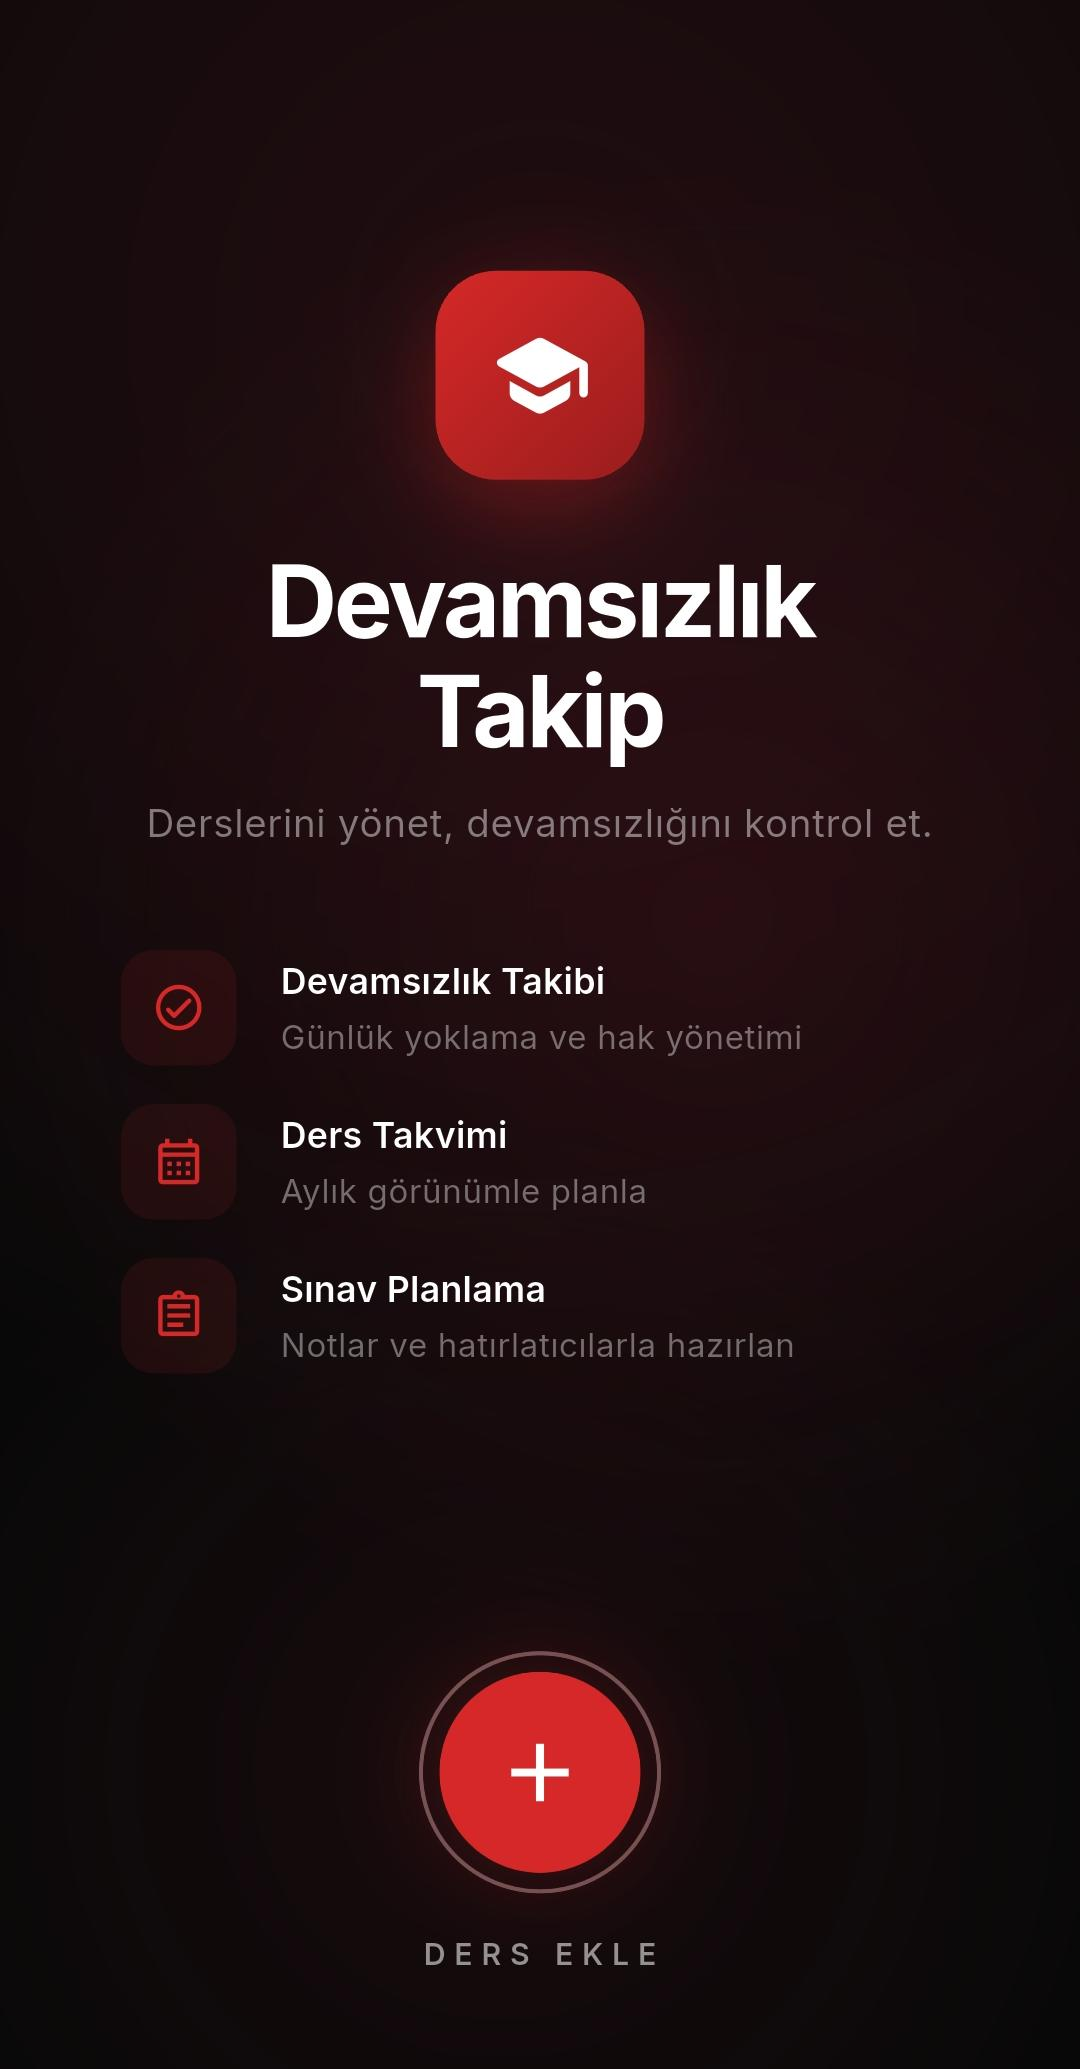
\includegraphics[height=9cm, keepaspectratio]{images/home_empty.jpeg}
    \caption{Boş Karşılama Ekranı: Aurora arka plan animasyonu ve Ders Ekle butonu}
    \label{fig:home_empty}
\end{figure}

\subsubsection{ANA Sekmesi — Günlük Yoklama}

Dersler eklendikten sonra ANA sekmesi iki bölüm sunar:

\textbf{BUGÜN} bölümü: O güne ait dersler saate göre sıralanmış kartlarda listelenir. Her kartta \textbf{GELDİM} (yeşil) ve \textbf{GELMEDİM} (kırmızı) aksiyon butonları bulunur.

\begin{figure}[H]
    \centering
    \begin{subfigure}[b]{0.42\textwidth}
        \centering
        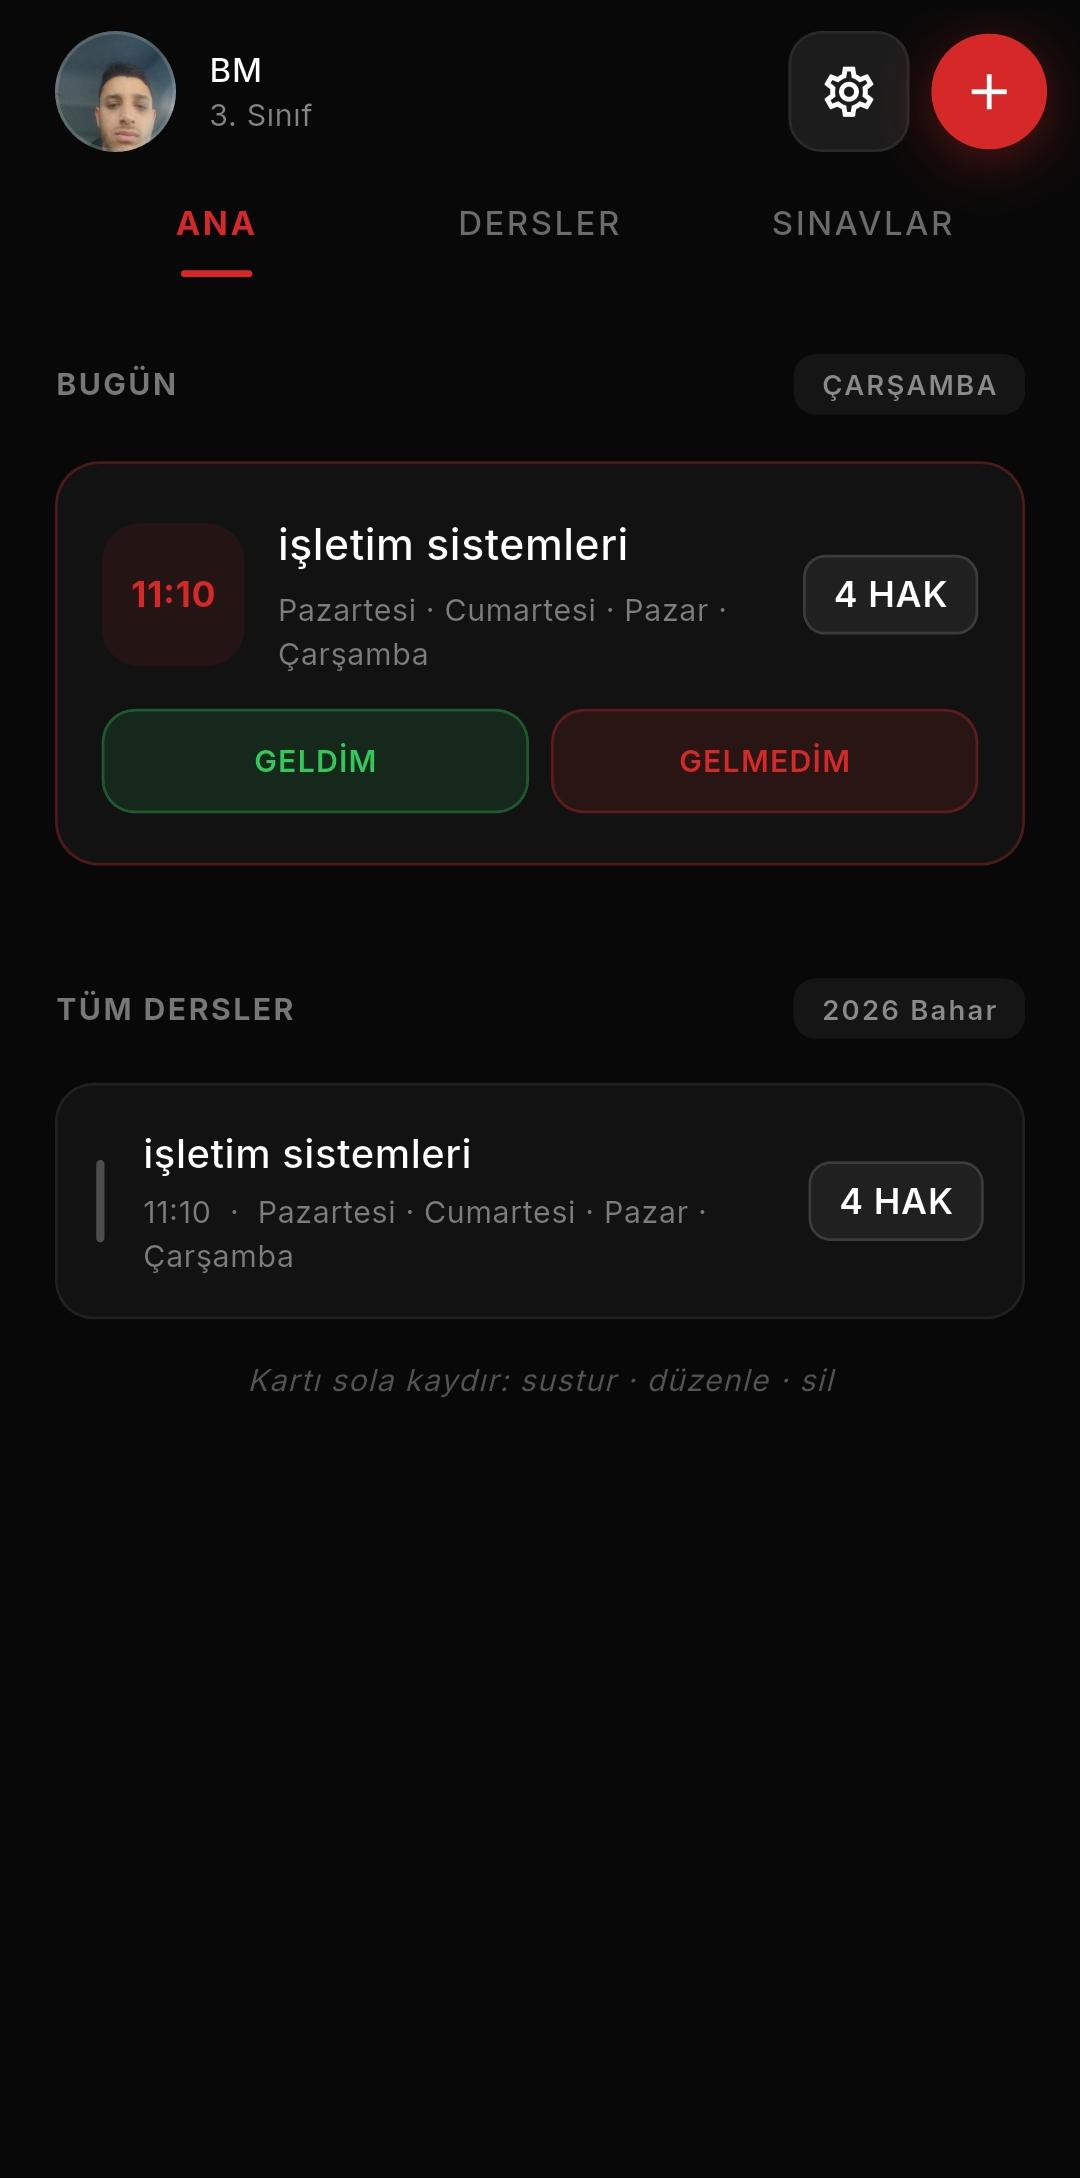
\includegraphics[height=8cm, keepaspectratio]{images/home_today.jpeg}
        \caption{İşaretlenmemiş ders kartları}
    \end{subfigure}
    \hfill
    \begin{subfigure}[b]{0.42\textwidth}
        \centering
        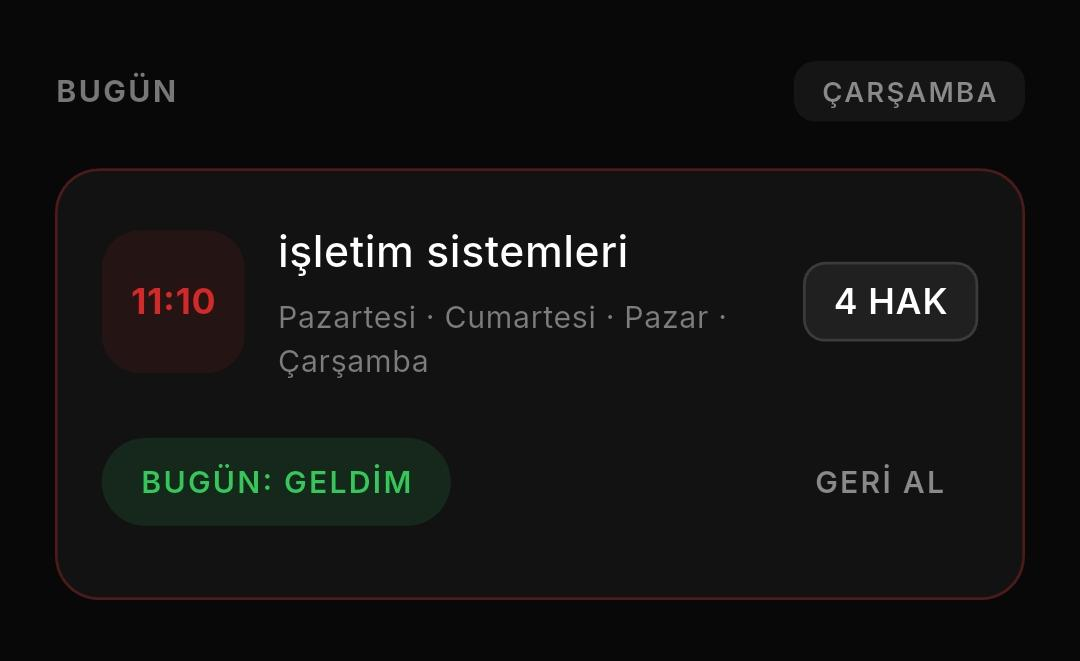
\includegraphics[height=8cm, keepaspectratio]{images/home_marked_geldim.jpeg}
        \caption{GELDİM işaretlendikten sonra}
    \end{subfigure}
    \caption{ANA Sekmesi BUGÜN Bölümü: Yoklama butonları ve işaretlenmiş durum}
    \label{fig:home_today}
\end{figure}

İşaretleme yapıldıktan sonra kart durum rozetine dönüşür ve \textbf{GERİ AL} butonu belirir. ``Gelmedim'' işaretlendiğinde dersin kalan hakkı otomatik olarak 1 azalır ve geri alındığında iade edilir.

\begin{figure}[H]
    \centering
    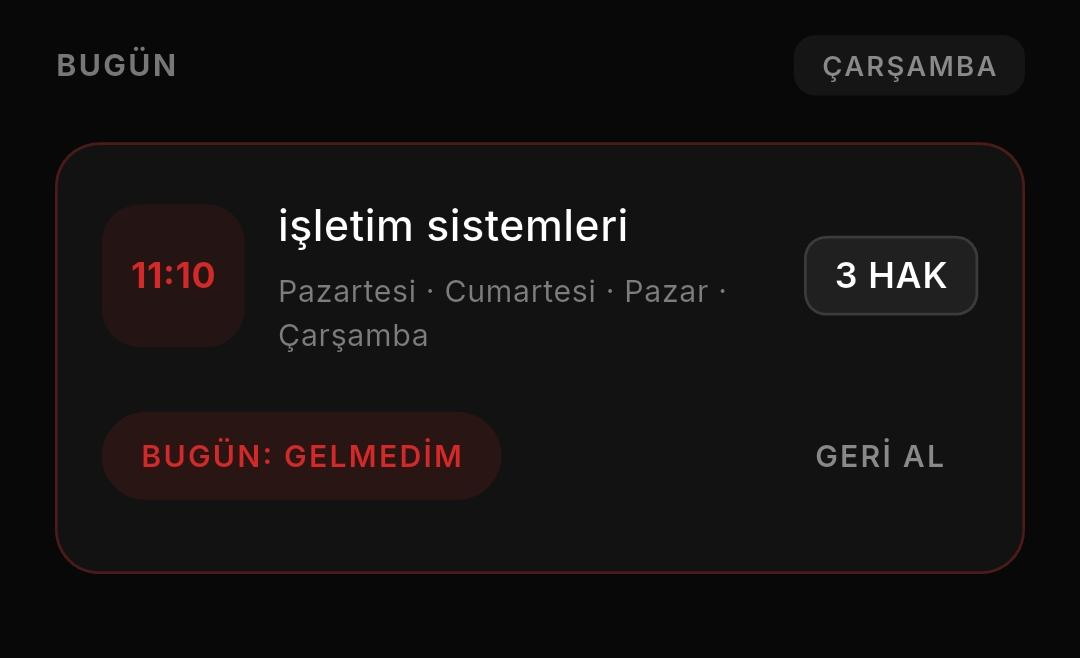
\includegraphics[height=9cm, keepaspectratio]{images/home_marked_gelmedim.jpeg}
    \caption{GELMEDİM işaretlenmiş kart: Kırmızı durum rozeti ve GERİ AL seçeneği}
    \label{fig:home_gelmedim}
\end{figure}

\textbf{TÜM DERSLER} bölümü: Dönemdeki tüm dersler kompakt kart formatında listelenir. Her kartta renkli sol bordür, ders saati, günler ve kalan hak rozeti yer alır.

\begin{figure}[H]
    \centering
    \begin{subfigure}[b]{0.42\textwidth}
        \centering
        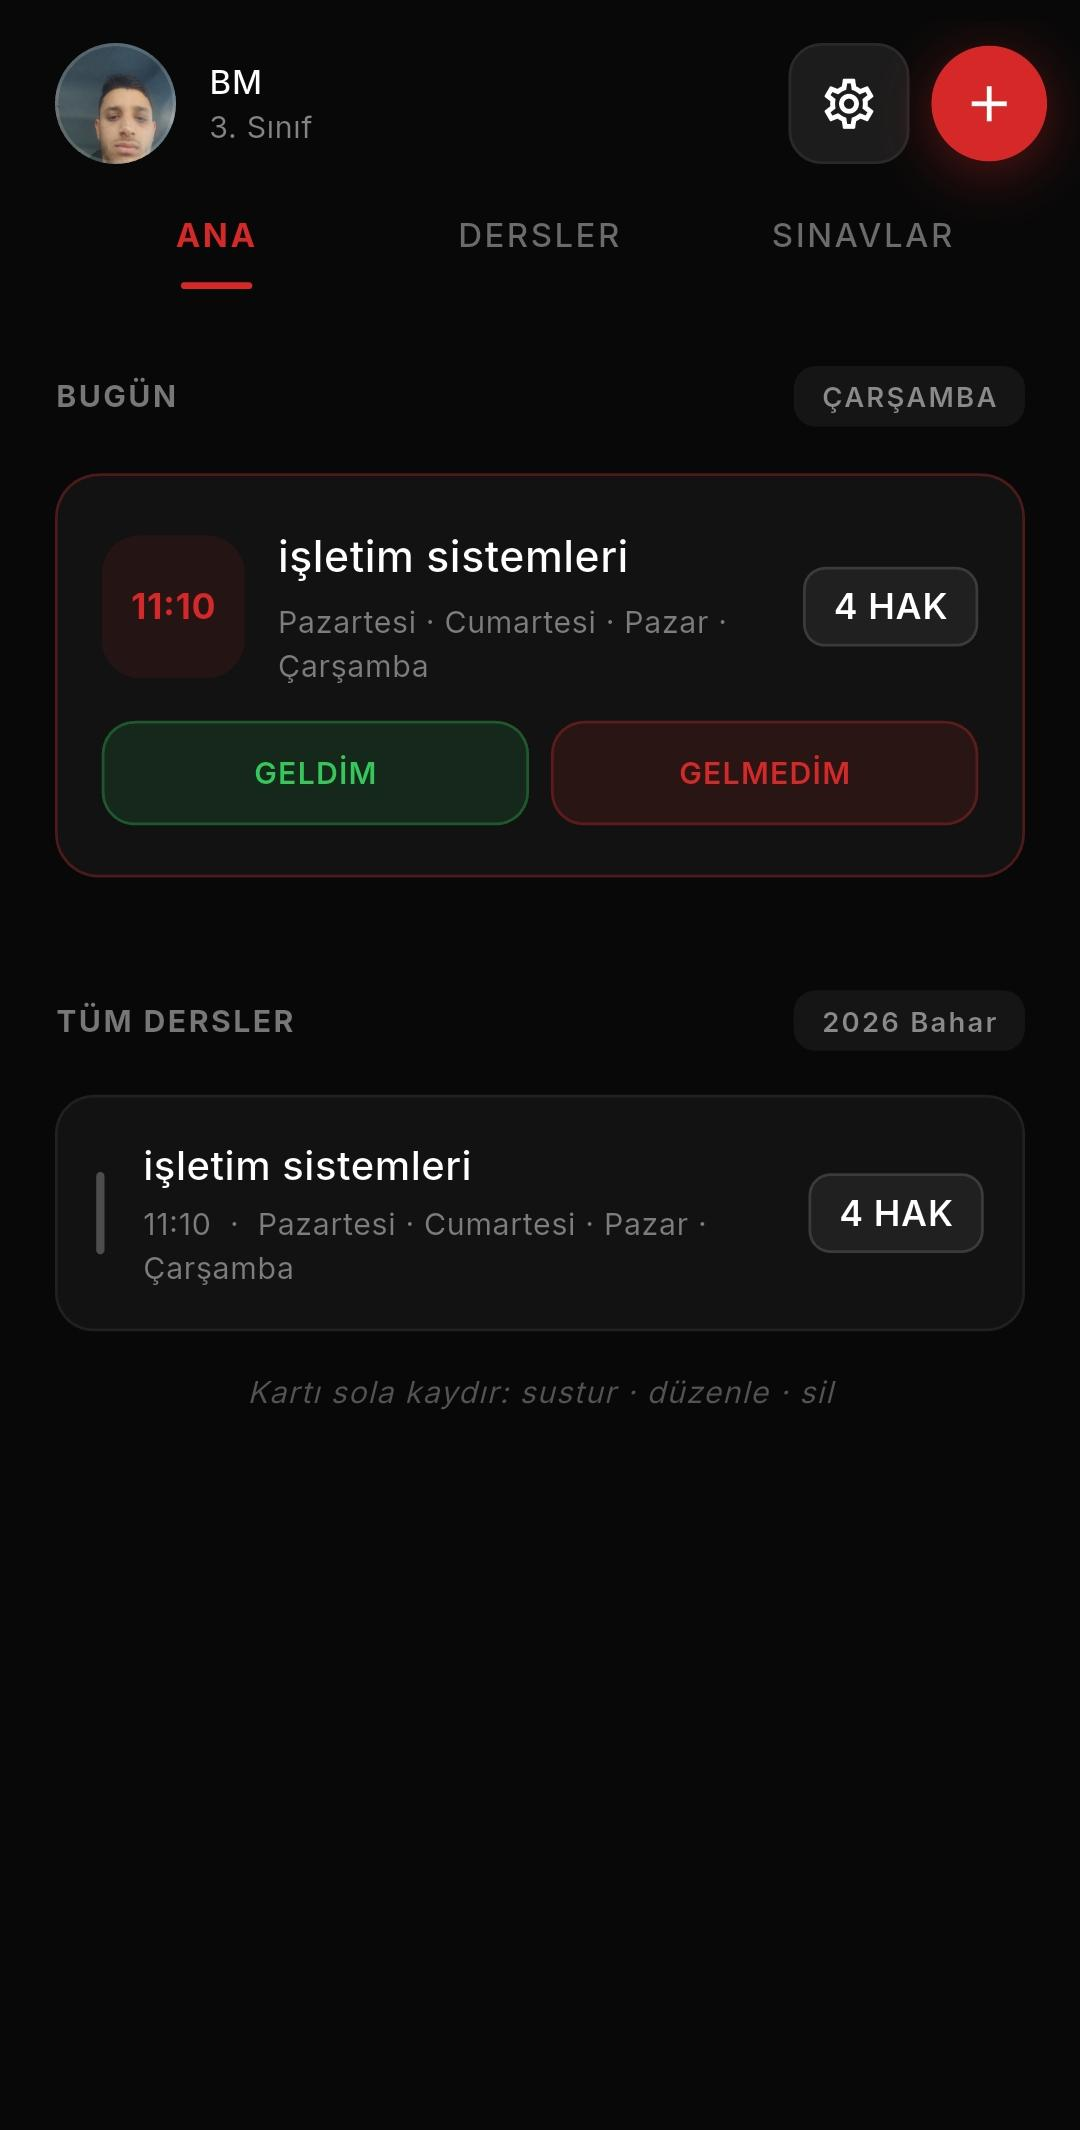
\includegraphics[height=8cm, keepaspectratio]{images/home_all_courses.jpeg}
        \caption{TÜM DERSLER bölümü}
    \end{subfigure}
    \hfill
    \begin{subfigure}[b]{0.42\textwidth}
        \centering
        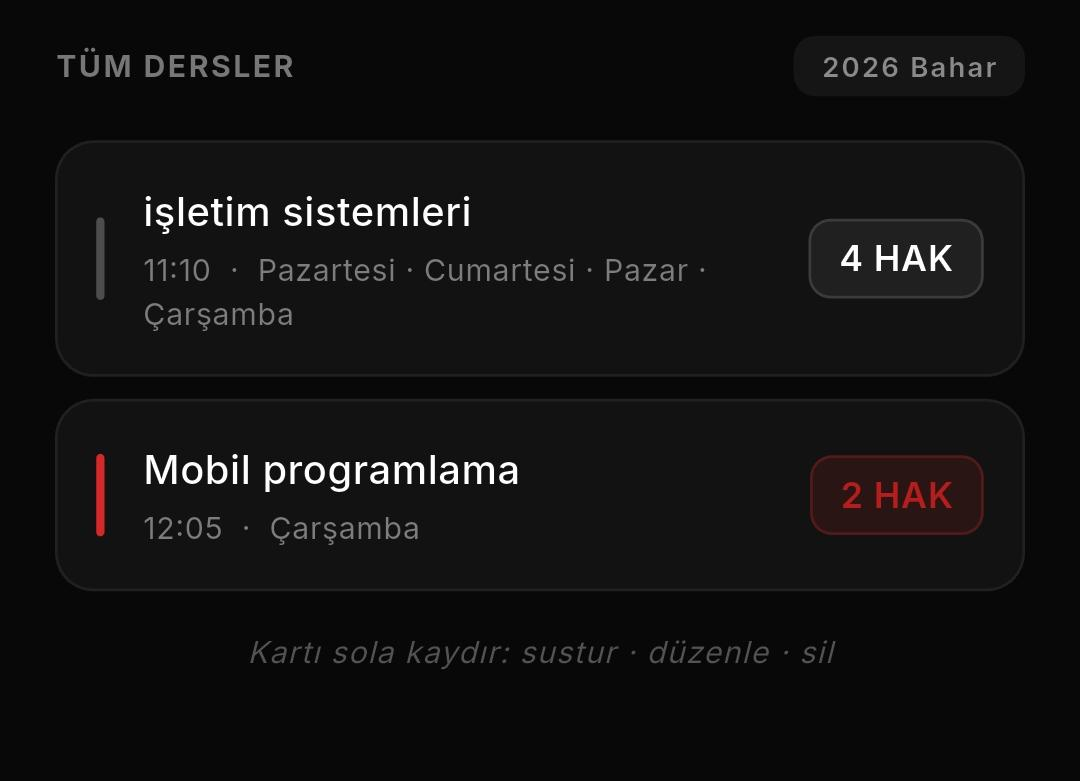
\includegraphics[height=8cm, keepaspectratio]{images/rights_critical.jpeg}
        \caption{Kritik hak uyarısı (≤2 hak)}
    \end{subfigure}
    \caption{Ders Kartları ve Devamsızlık Hakkı Rozeti}
    \label{fig:all_courses}
\end{figure}

\textbf{Kaydırma Aksiyonları:} Herhangi bir ders kartı sola kaydırıldığında \texttt{flutter\_slidable} ile üç gizli aksiyon ortaya çıkar: \textbf{Sustur/Aç} (bildirim yönetimi), \textbf{Düzenle} ve \textbf{Sil}.

\begin{figure}[H]
    \centering
    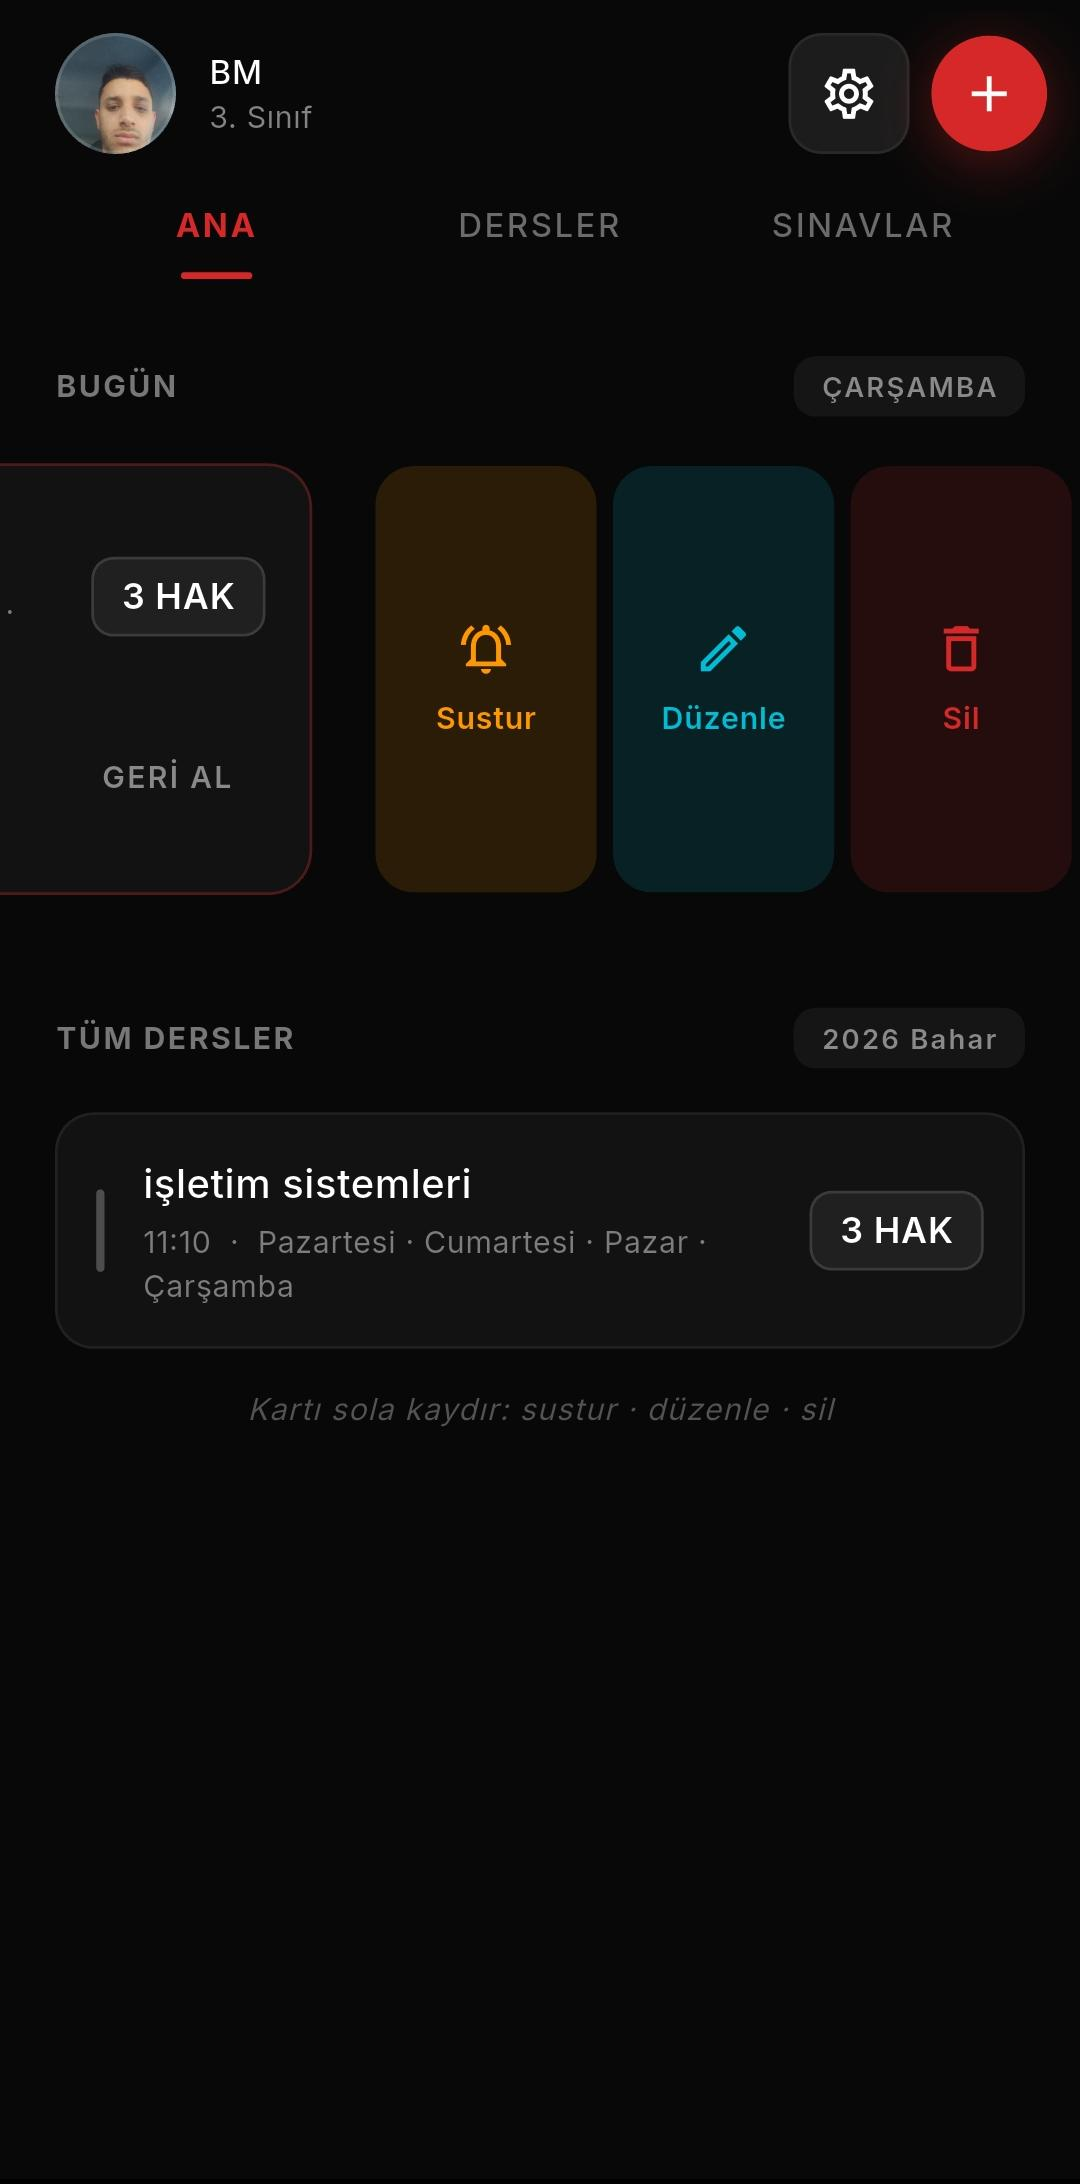
\includegraphics[height=9cm, keepaspectratio]{images/home_swipe.jpeg}
    \caption{Kaydırma Aksiyonları: Sustur, Düzenle ve Sil seçenekleri}
    \label{fig:swipe}
\end{figure}

\subsubsection{DERSLER Sekmesi — Ders Takvimi}

\texttt{table\_calendar} paketi ile aylık takvim görünümü sunar. Her günün altında o güne ait dersler \textbf{renkli noktalarla} işaretlenir (en fazla 6 nokta, 3'erli iki sıra). Bugün kırmızı çemberle, seçili gün açık kırmızı tonla vurgulanır.

\begin{figure}[H]
    \centering
    \begin{subfigure}[b]{0.42\textwidth}
        \centering
        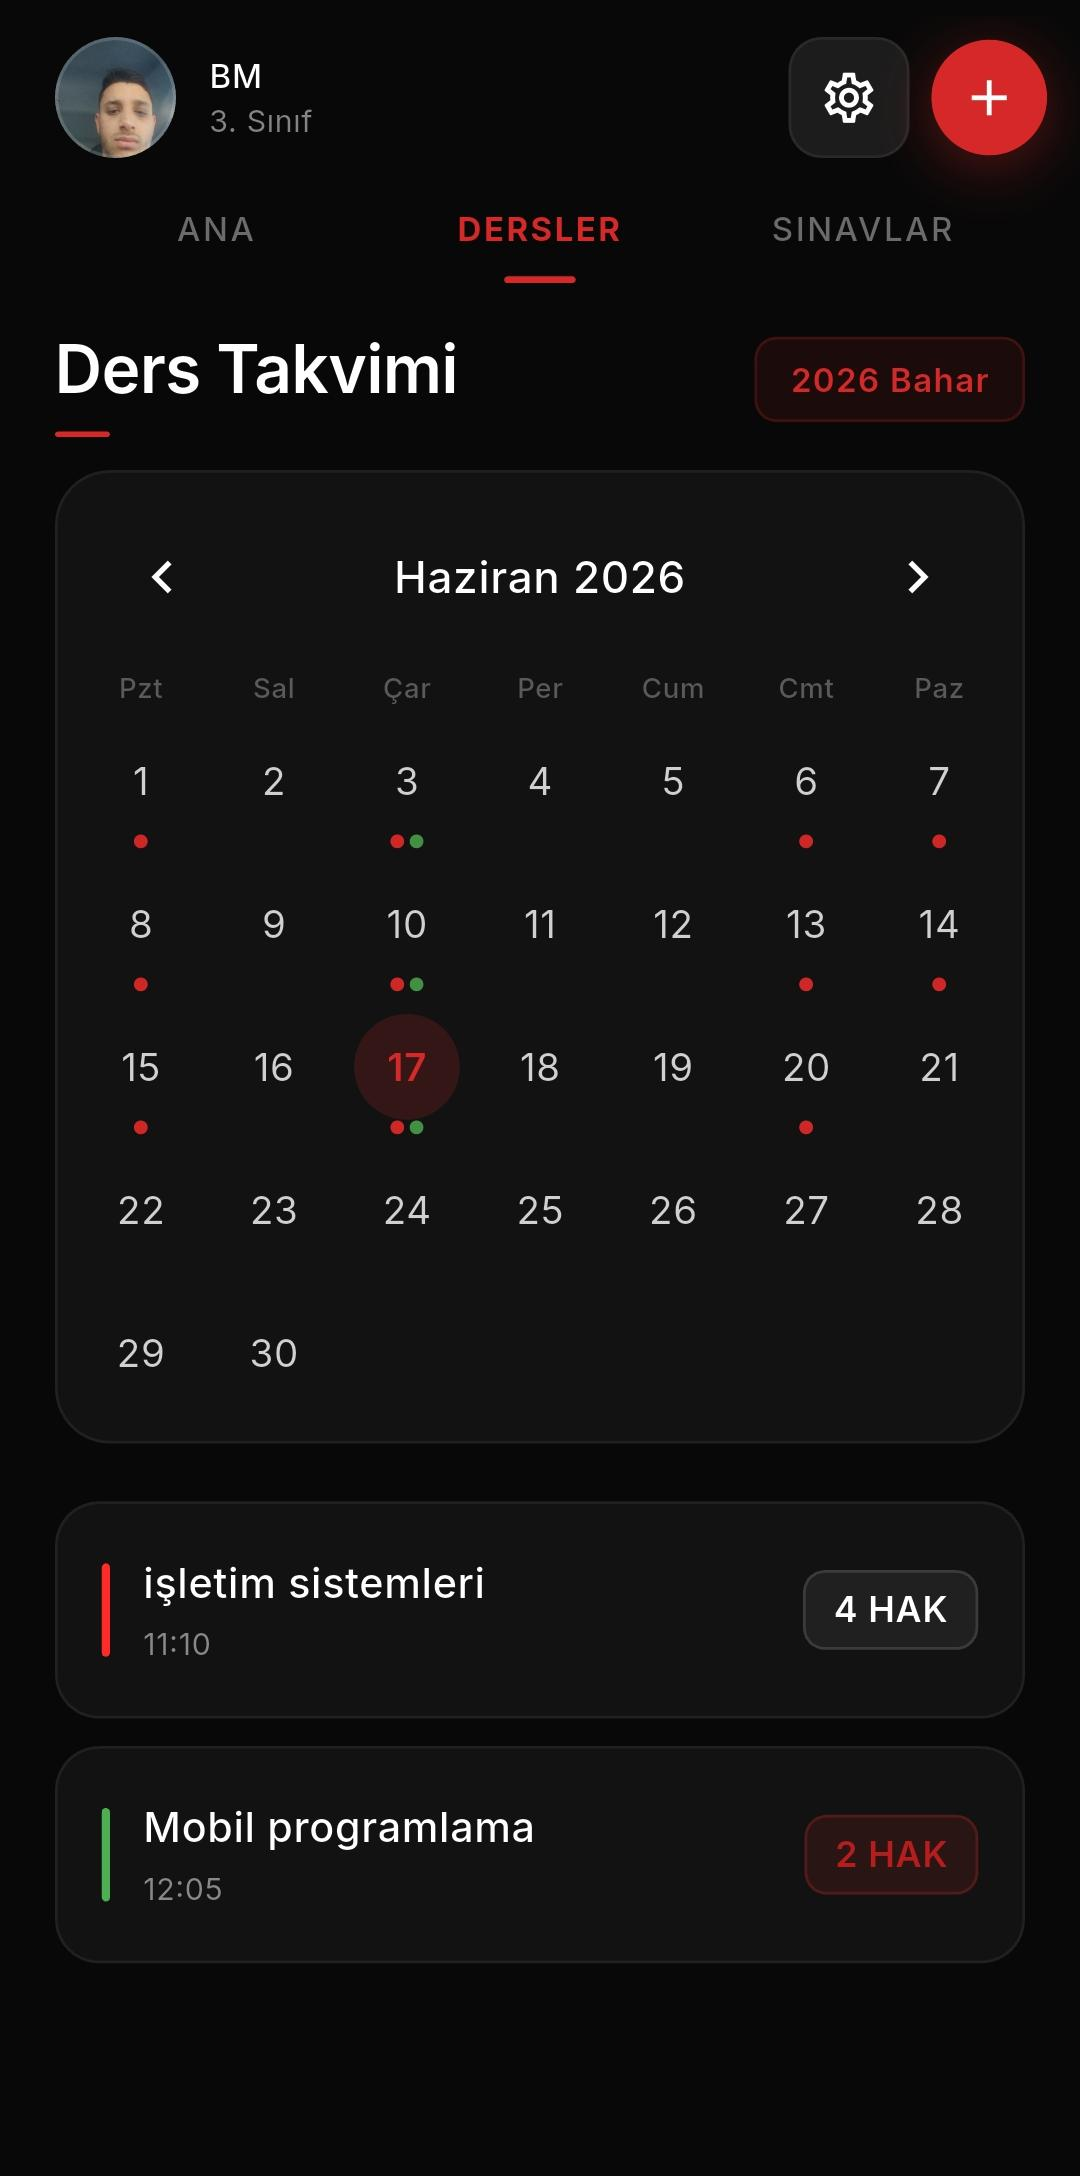
\includegraphics[height=8cm, keepaspectratio]{images/calendar_dots.jpeg}
        \caption{Renkli noktalı takvim görünümü}
    \end{subfigure}
    \hfill
    \begin{subfigure}[b]{0.42\textwidth}
        \centering
        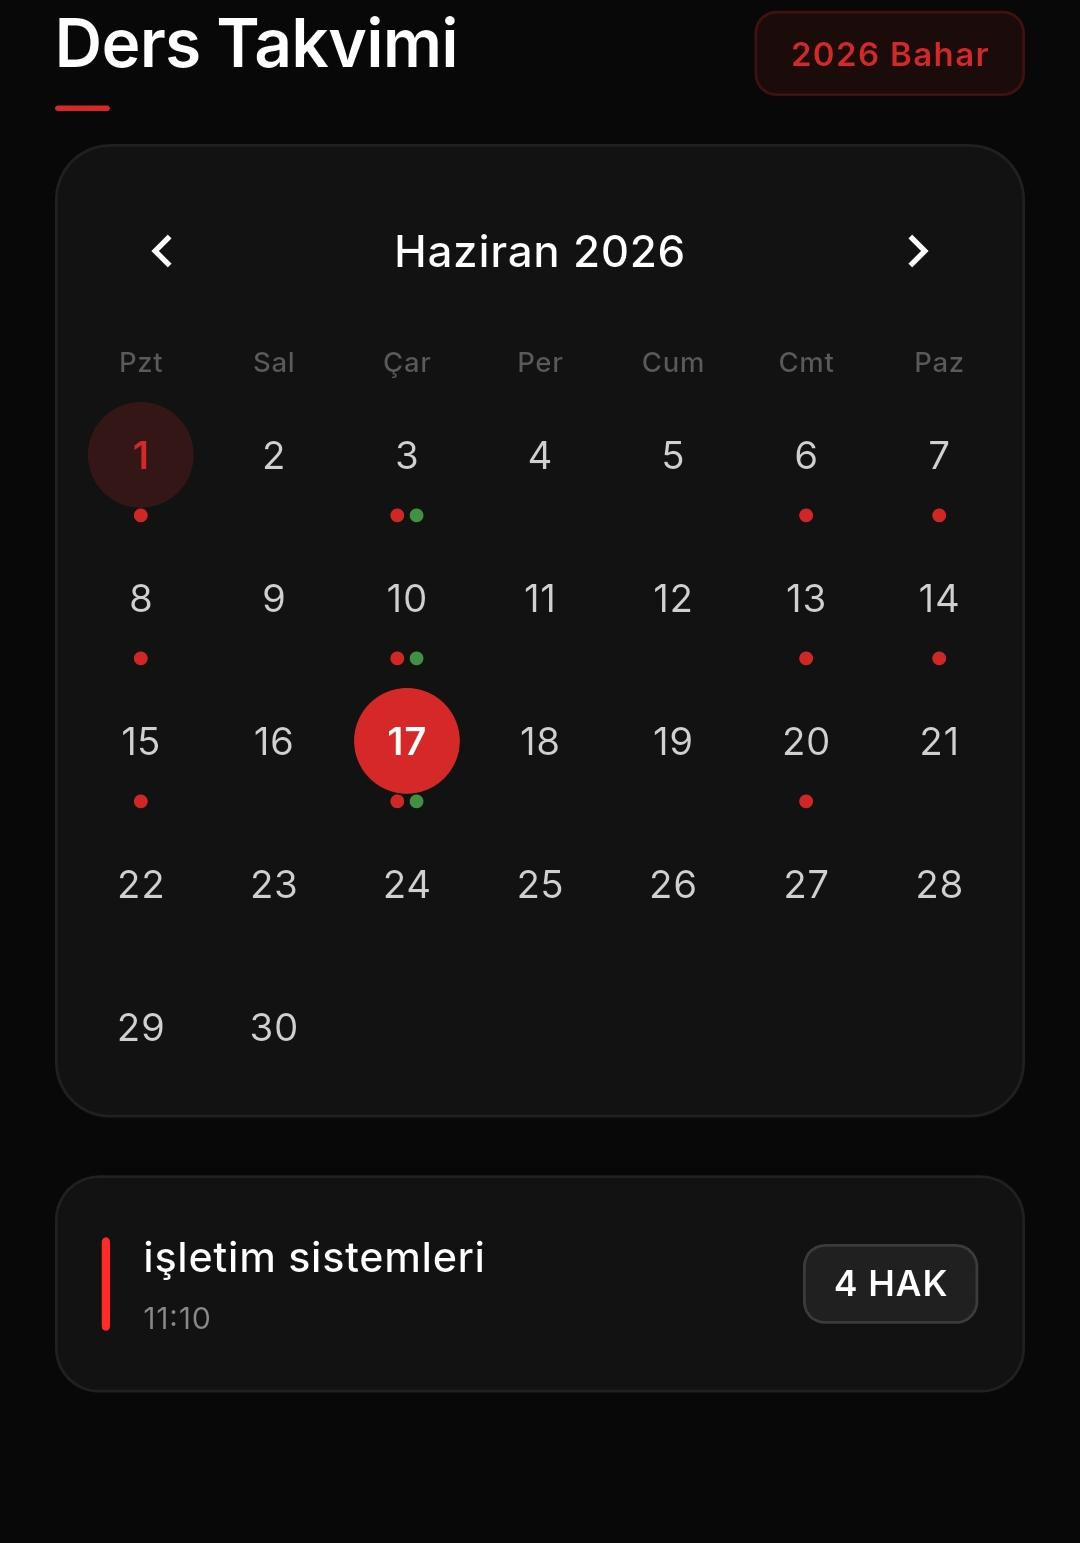
\includegraphics[height=8cm, keepaspectratio]{images/calendar_day.jpeg}
        \caption{Seçili gün ders detayları}
    \end{subfigure}
    \caption{Ders Takvimi Ekranı: Renkli noktalar ve gün detayı paneli}
    \label{fig:calendar}
\end{figure}

Bir güne dokunulduğunda o günün ders listesi, kalan hakları ve yoklama durumlarıyla birlikte altta görüntülenir. Resmi tatil günlerinde mavi \textbf{``T''} göstergesi ve tatil adı gösterilir; dönem dışı günlerde ders listesi boş bırakılır.

\begin{figure}[H]
    \centering
    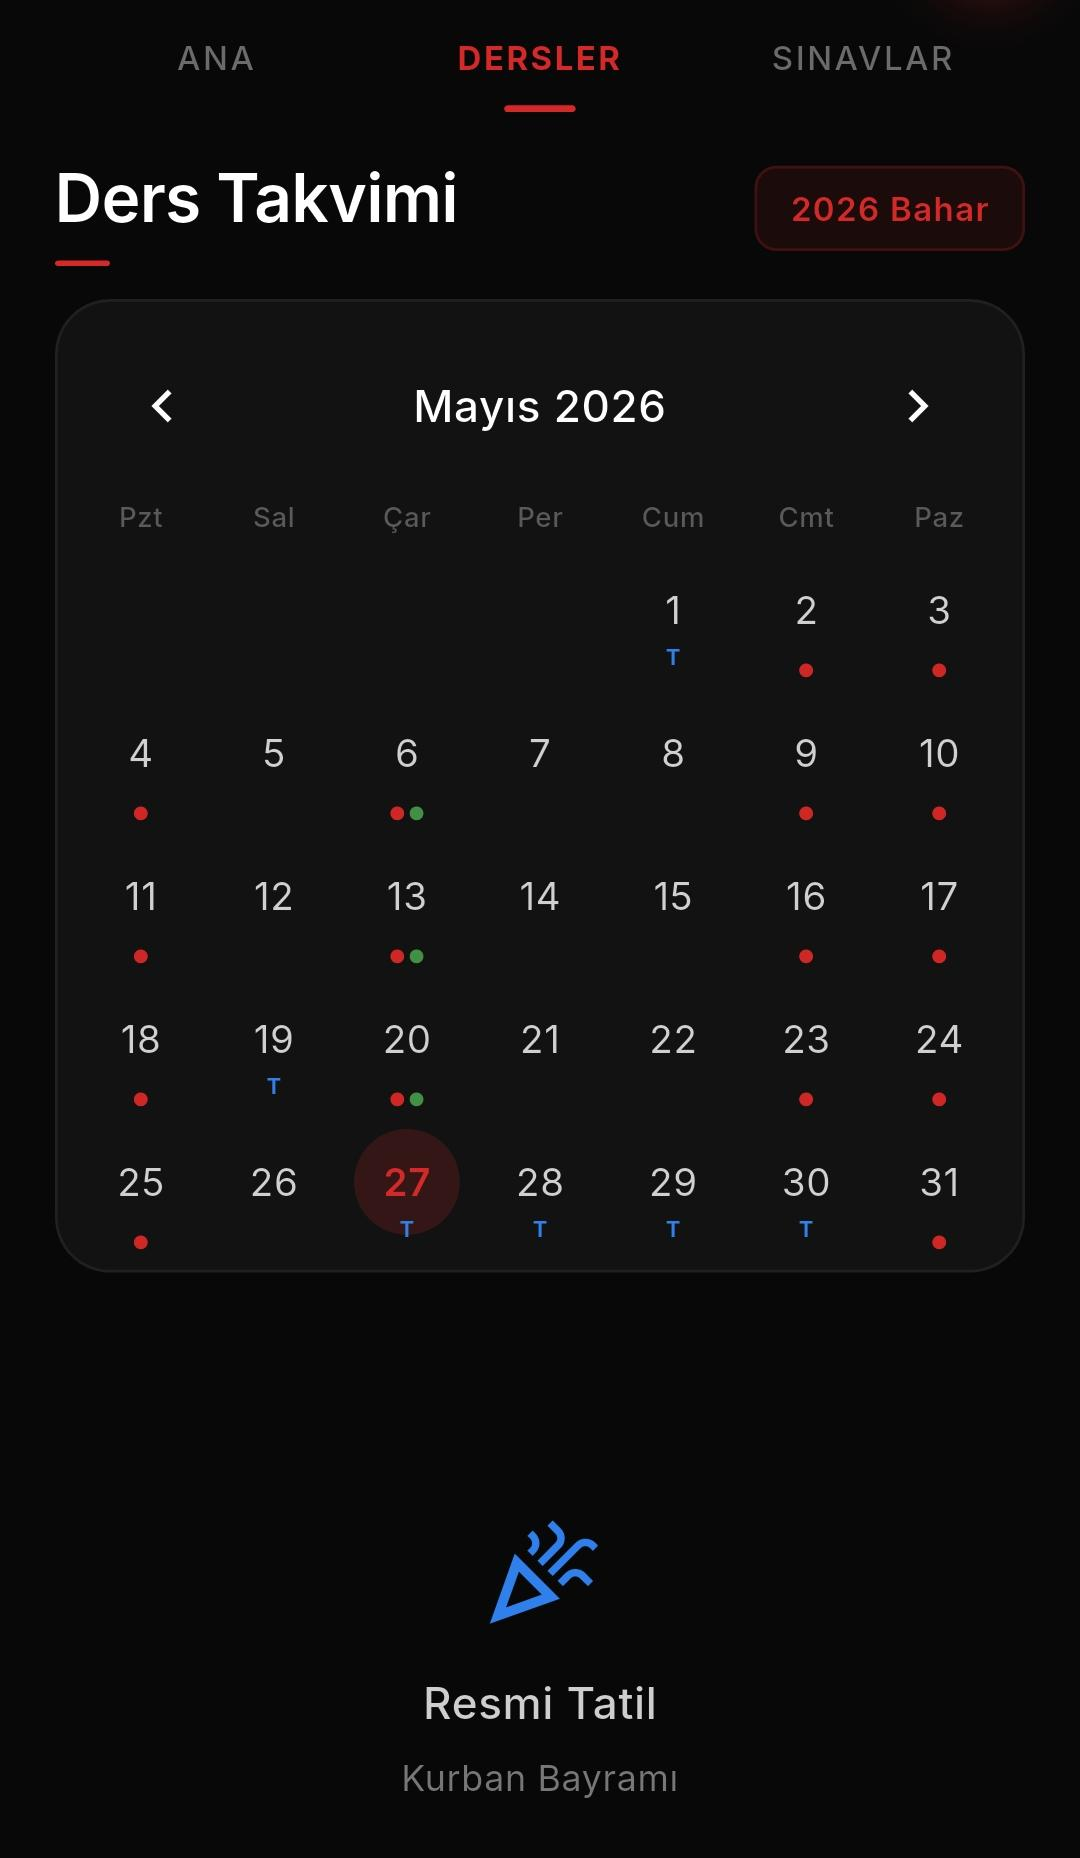
\includegraphics[height=9cm, keepaspectratio]{images/calendar_holiday.jpeg}
    \caption{Tatil Günü Gösterimi: Mavi T işareti ve tatil adı}
    \label{fig:holiday}
\end{figure}

\subsubsection{SINAVLAR Sekmesi — Sınav Takvimi}

\textbf{Dosya:} \texttt{features/exams/exam\_calendar\_screen.dart}

Sınav takibine ayrılmış iki alt sekme sunar. Renk aksanı ders takviminin kırmızısından ayrışmak için \textbf{indigo} olarak belirlenmiştir.

\begin{figure}[H]
    \centering
    \begin{subfigure}[b]{0.42\textwidth}
        \centering
        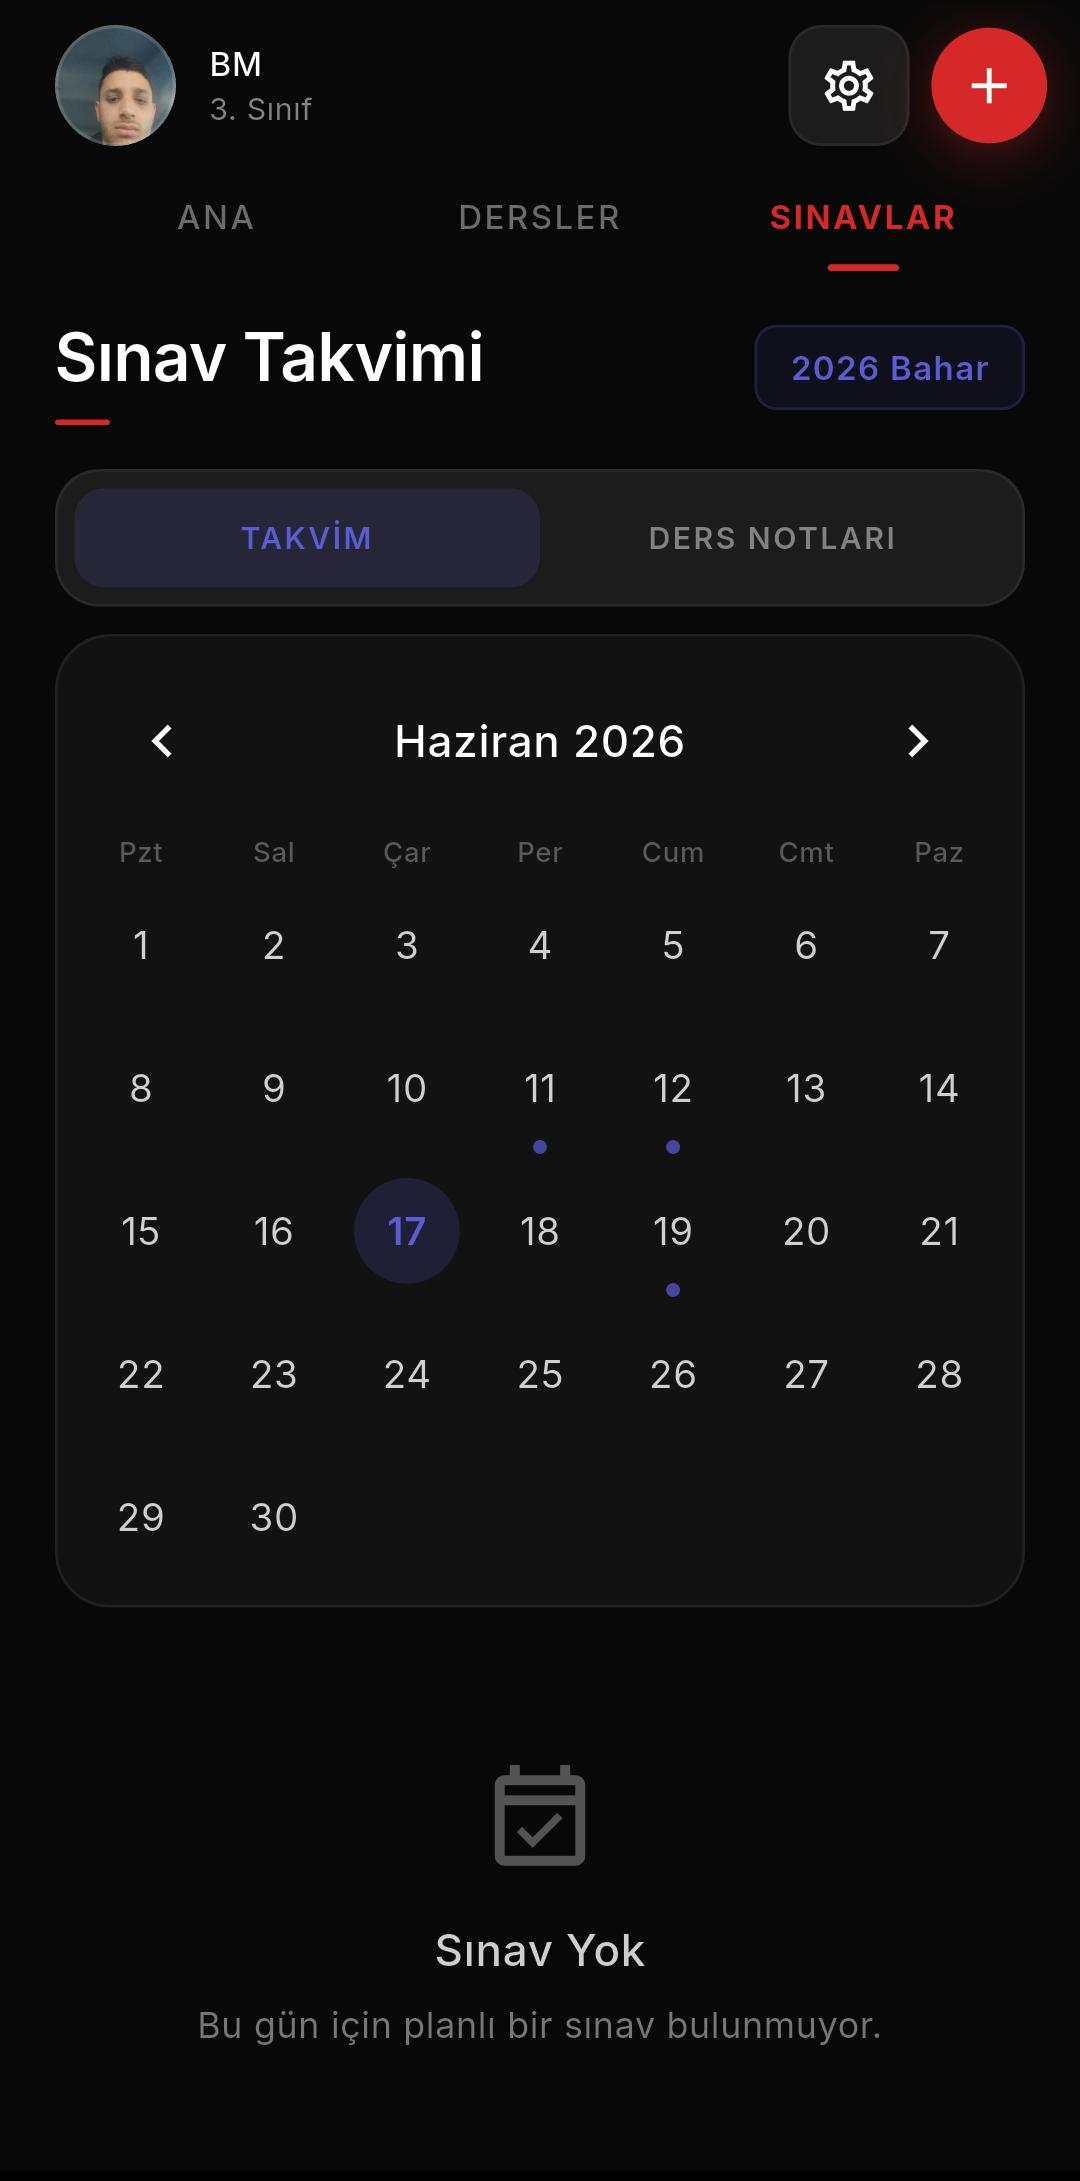
\includegraphics[height=8cm, keepaspectratio]{images/exam_calendar.jpeg}
        \caption{TAKVİM alt sekmesi}
    \end{subfigure}
    \hfill
    \begin{subfigure}[b]{0.42\textwidth}
        \centering
        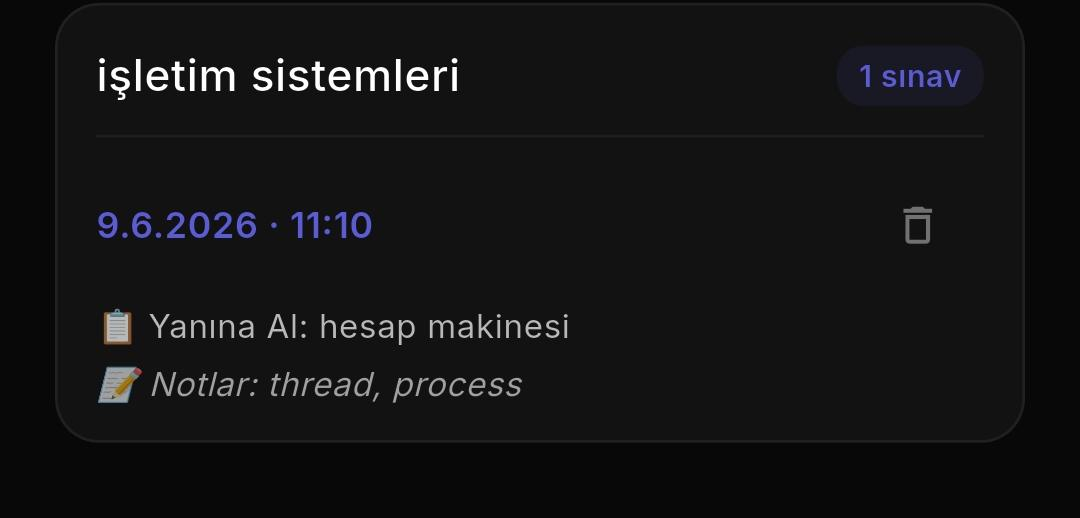
\includegraphics[height=8cm, keepaspectratio]{images/exam_notes.jpeg}
        \caption{DERS NOTLARI alt sekmesi}
    \end{subfigure}
    \caption{Sınav Takvimi Ekranı: Takvim görünümü ve ders notları}
    \label{fig:exam_cal}
\end{figure}

\begin{description}
    \item[TAKVİM] Sınav günleri indigo nokta işaretçileriyle gösterilir. Seçili günün sınavları saat, ``yanına al'' listesi ve notlarıyla birlikte listelenir; silebilir.
    \item[DERS NOTLARI] Sınavlar ders bazında gruplanır. Her ders başlığı altında sınav tarihleri, saatleri, notlar ve yanına al listesi düzenli şekilde sunulur.
\end{description}

\subsection{Ders Ekleme / Düzenleme Ekranı}
\textbf{Dosya:} \texttt{features/schedule/add\_course\_screen.dart}

Yeni ders eklemek veya mevcut dersi düzenlemek için kullanılır. \texttt{existing} parametresi \texttt{null} ise ekleme modu, dolu ise düzenleme modu aktiftir. Formun bölümleri kademeli animasyonla (alt-üst kayma + solma, toplam \textasciitilde{}600ms) belirir.

\begin{figure}[H]
    \centering
    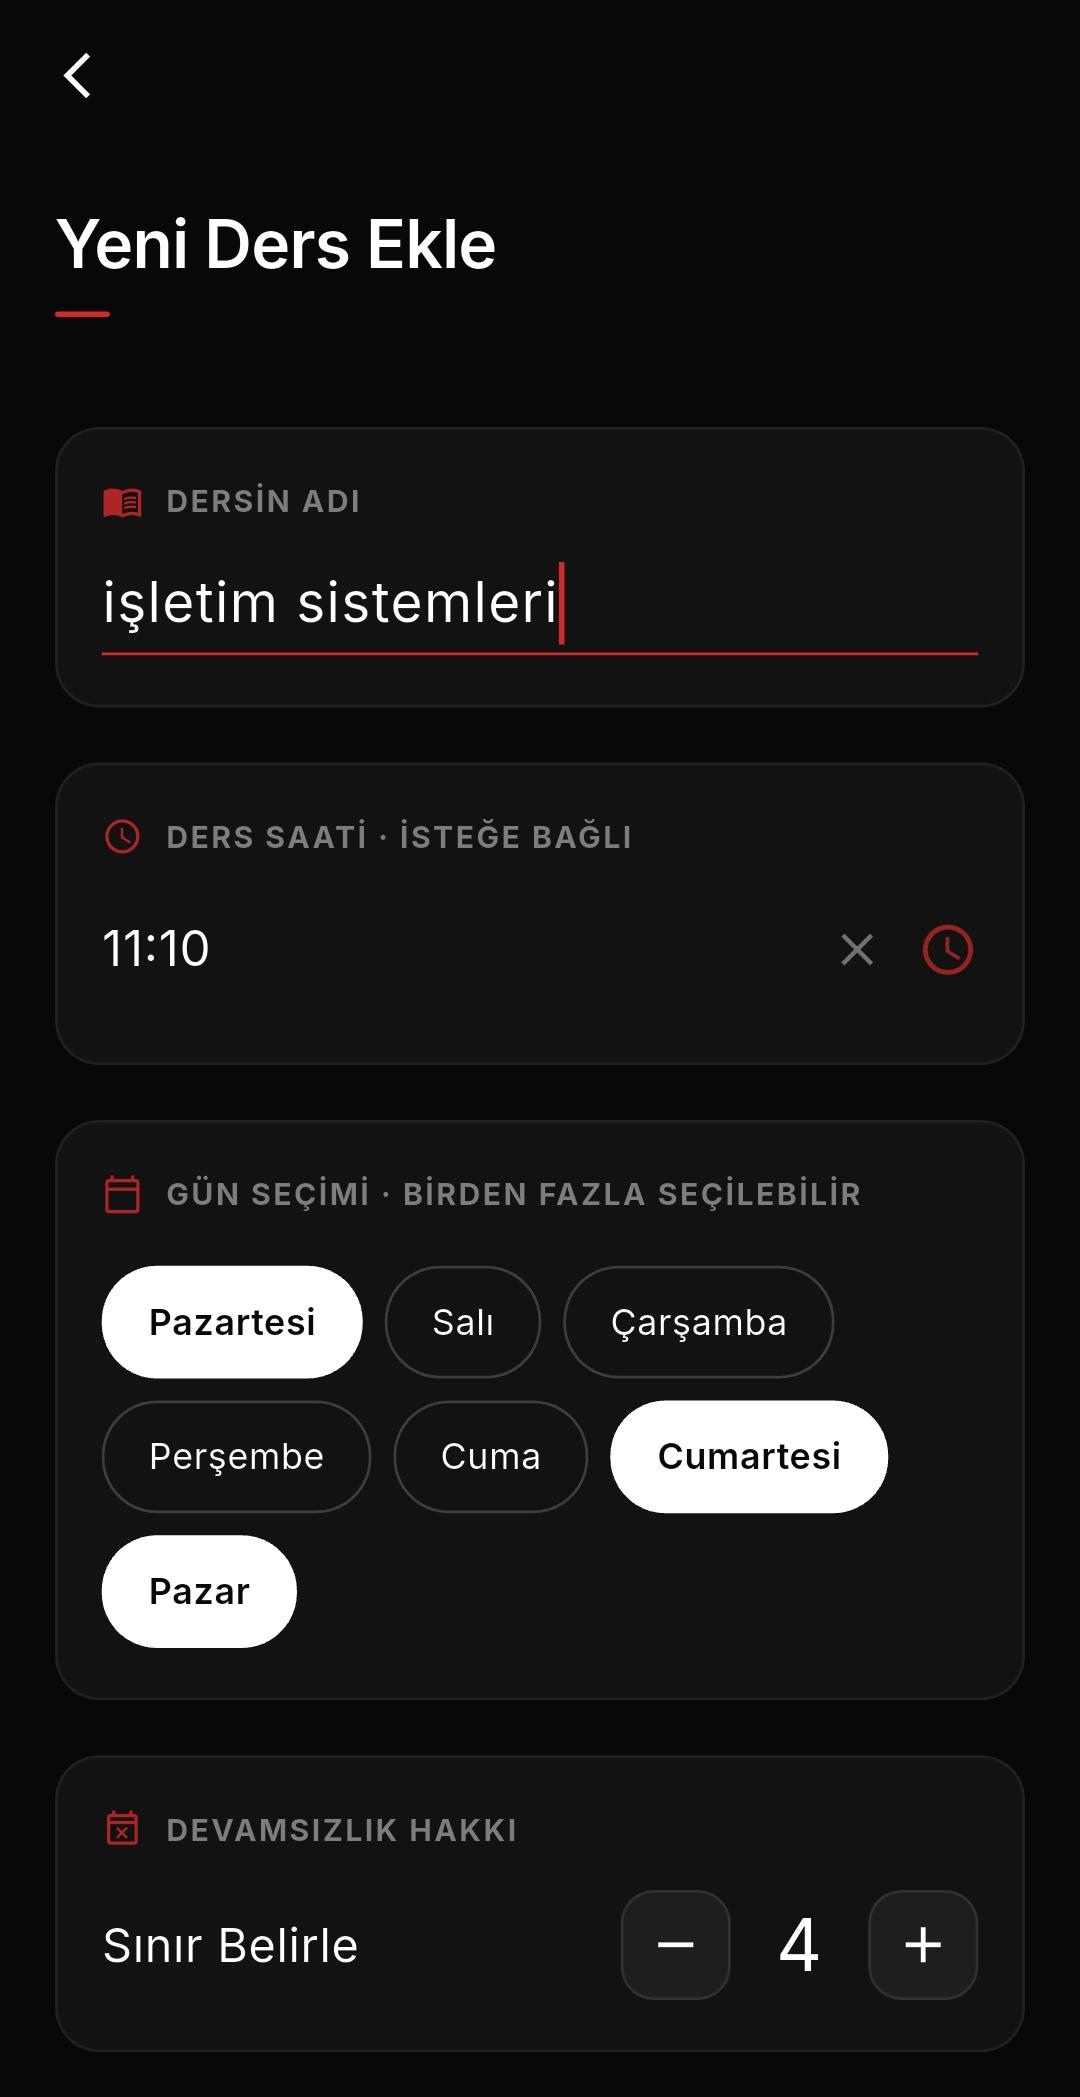
\includegraphics[height=9cm, keepaspectratio]{images/add_course.jpeg}
    \caption{Ders Ekleme Ekranı: Form alanları ve gün seçici}
    \label{fig:add_course}
\end{figure}

Form alanları:
\begin{enumerate}
    \item \textbf{DERSİN ADI} --- Metin girişi, maksimum 40 karakter.
    \item \textbf{DERS SAATİ} --- İsteğe bağlı; seçilen dakika değeri en yakın 5'e yuvarlanır.
    \item \textbf{GÜN SEÇİMİ} --- Çoklu seçim; haftanın 7 günü pill/etiket olarak gösterilir; seçili olanlar dolgu rengiyle işaretlenir.
    \item \textbf{DEVAMSIZLIK HAKKI} --- +/- sayaç ile belirlenir; varsayılan değer 4'tür.
\end{enumerate}

\textbf{Doğrulama Kuralları:}
\begin{itemize}
    \item Ders adı boş bırakılamaz.
    \item En az bir gün seçilmesi zorunludur.
    \item Aynı dönemdeki aynı isimli ders engellenmiştir (Türkçe karakter duyarlı: İ$\leftrightarrow$i, I$\leftrightarrow$ı).
    \item Bir güne en fazla 6 ders eklenebilir.
\end{itemize}

\subsection{Sınav Ekleme Ekranı}
\textbf{Dosya:} \texttt{features/exams/exam\_add\_screen.dart}

Sınav ekleme arayüzü \textbf{sürükle-bırak (drag \& drop)} etkileşimi üzerine kuruludur. Dönemdeki dersler ekranın üst şeridinde sürüklenebilir etiket (Draggable) olarak listelenir; kullanıcı bir dersi takvimde istediği güne sürükler.

\begin{figure}[H]
    \centering
    \begin{subfigure}[b]{0.42\textwidth}
        \centering
        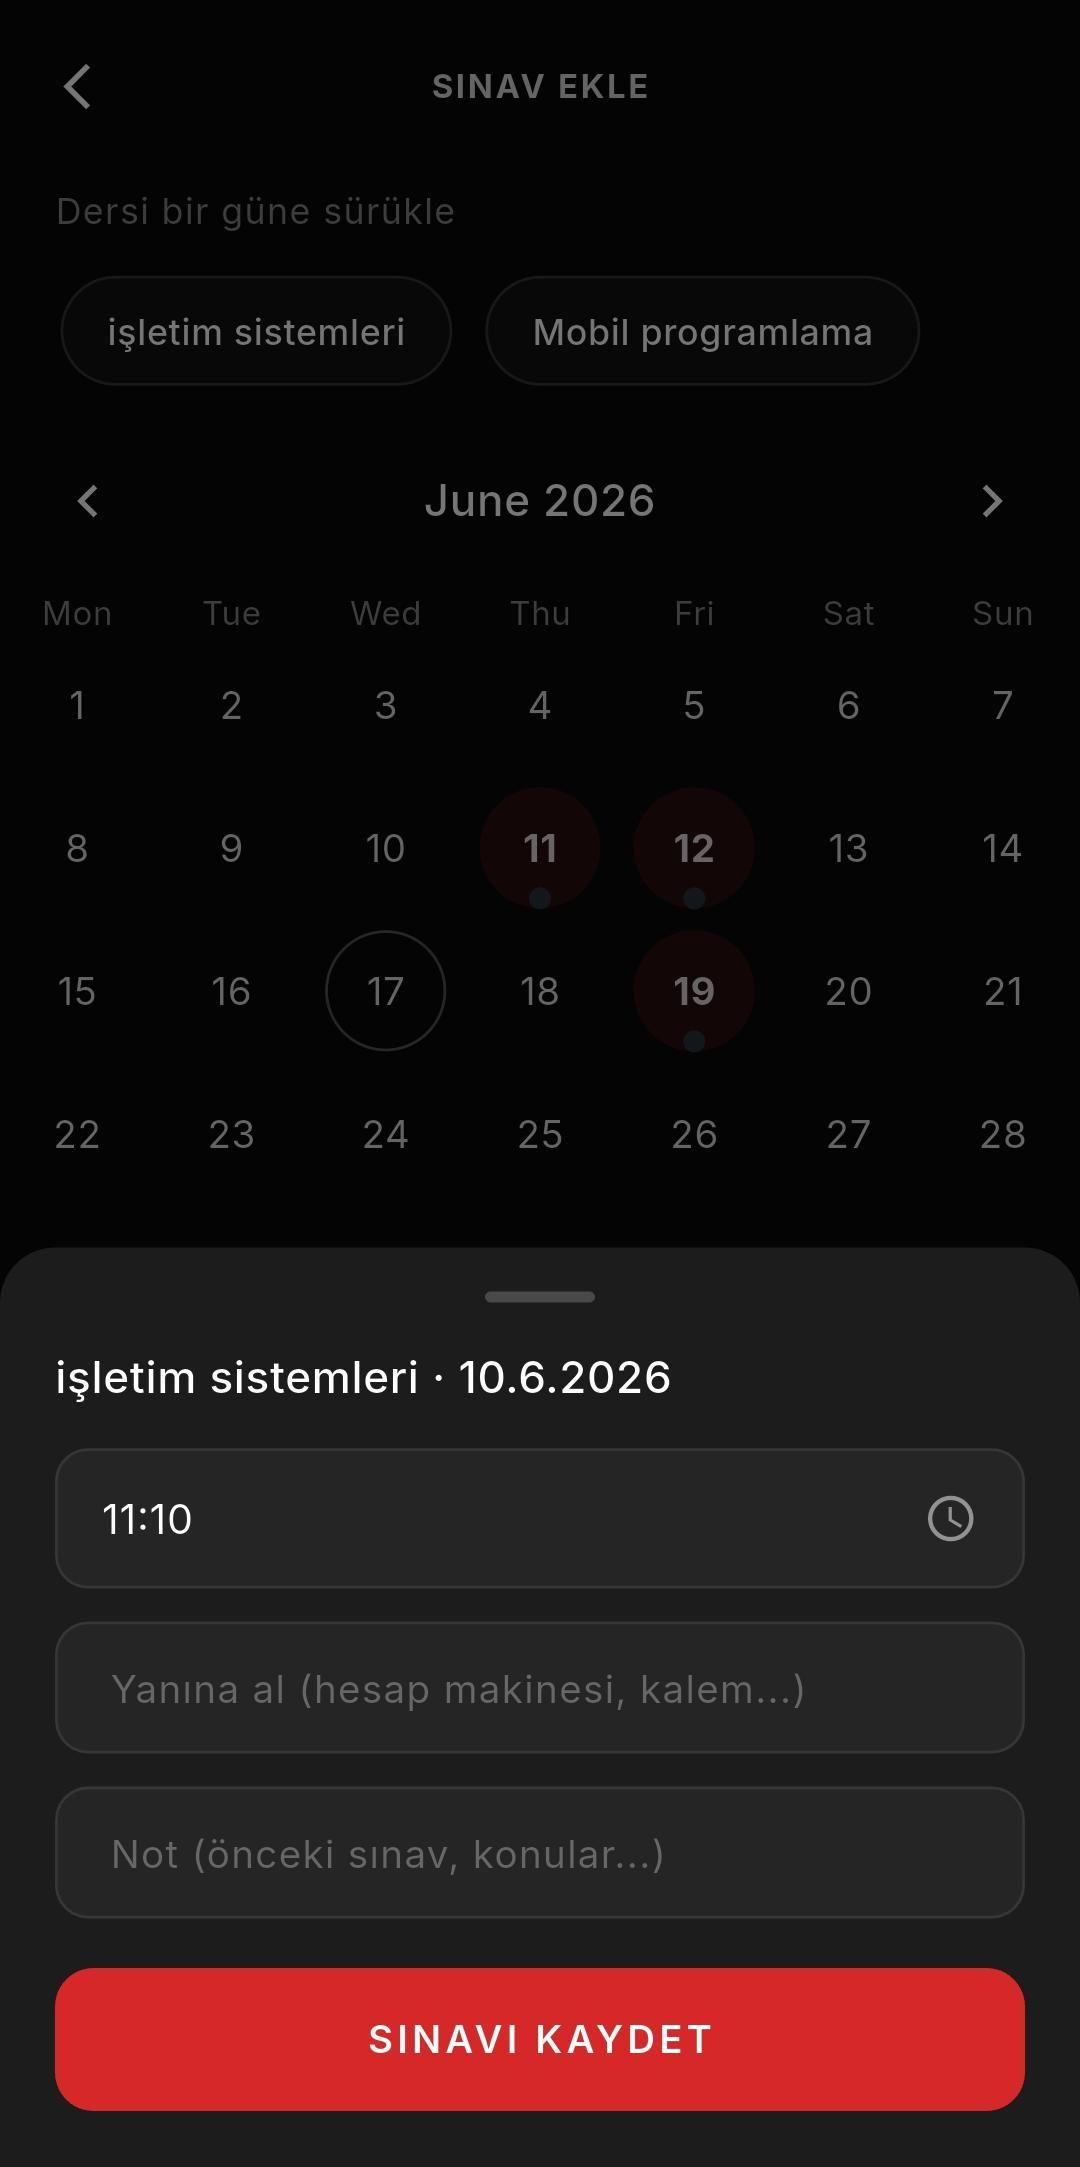
\includegraphics[height=8cm, keepaspectratio]{images/exam_add.jpeg}
        \caption{Sürükle-bırak arayüzü}
    \end{subfigure}
    \hfill
    \begin{subfigure}[b]{0.42\textwidth}
        \centering
        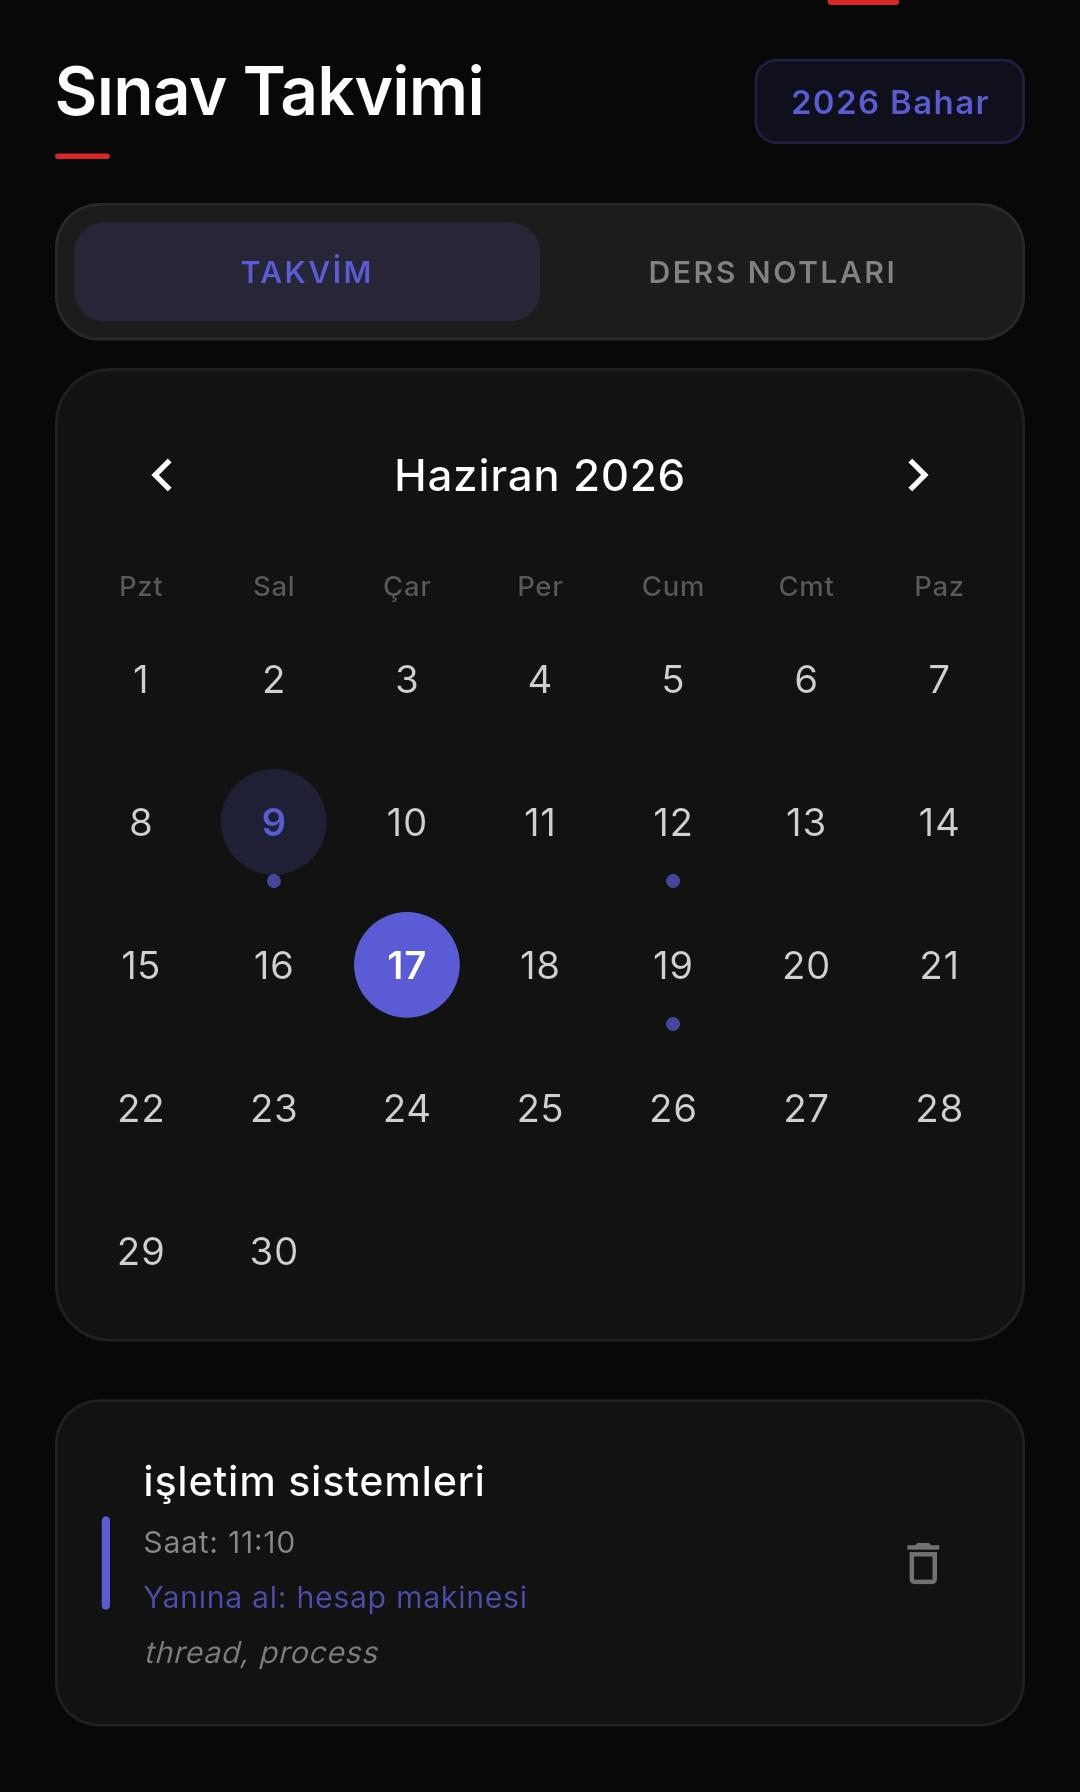
\includegraphics[height=8cm, keepaspectratio]{images/exam_detail.jpeg}
        \caption{Sınav detay alt paneli}
    \end{subfigure}
    \caption{Sınav Ekleme: Sürükle-bırak ve detay giriş paneli}
    \label{fig:exam_add}
\end{figure}

Ders bir güne bırakıldığında alt panel (bottom sheet) açılır ve kullanıcı şu bilgileri girebilir:
\begin{itemize}
    \item \textbf{Sınav Saati} --- İsteğe bağlı saat seçimi.
    \item \textbf{Yanına Al} --- Sınava götürülecek malzeme listesi (kalem, hesap makinesi vb.).
    \item \textbf{Not} --- Konu bilgisi, geçmiş sınav sonuçları veya hatırlatıcılar.
\end{itemize}

Aynı derse aynı güne ikinci sınav eklenmesini engelleyen çift kayıt doğrulaması mevcuttur.

\subsection{Profil Ekranı}
\textbf{Dosya:} \texttt{features/profile/profile\_screen.dart}

Öğrenci bilgilerini düzenleme ekranıdır.

\begin{figure}[H]
    \centering
    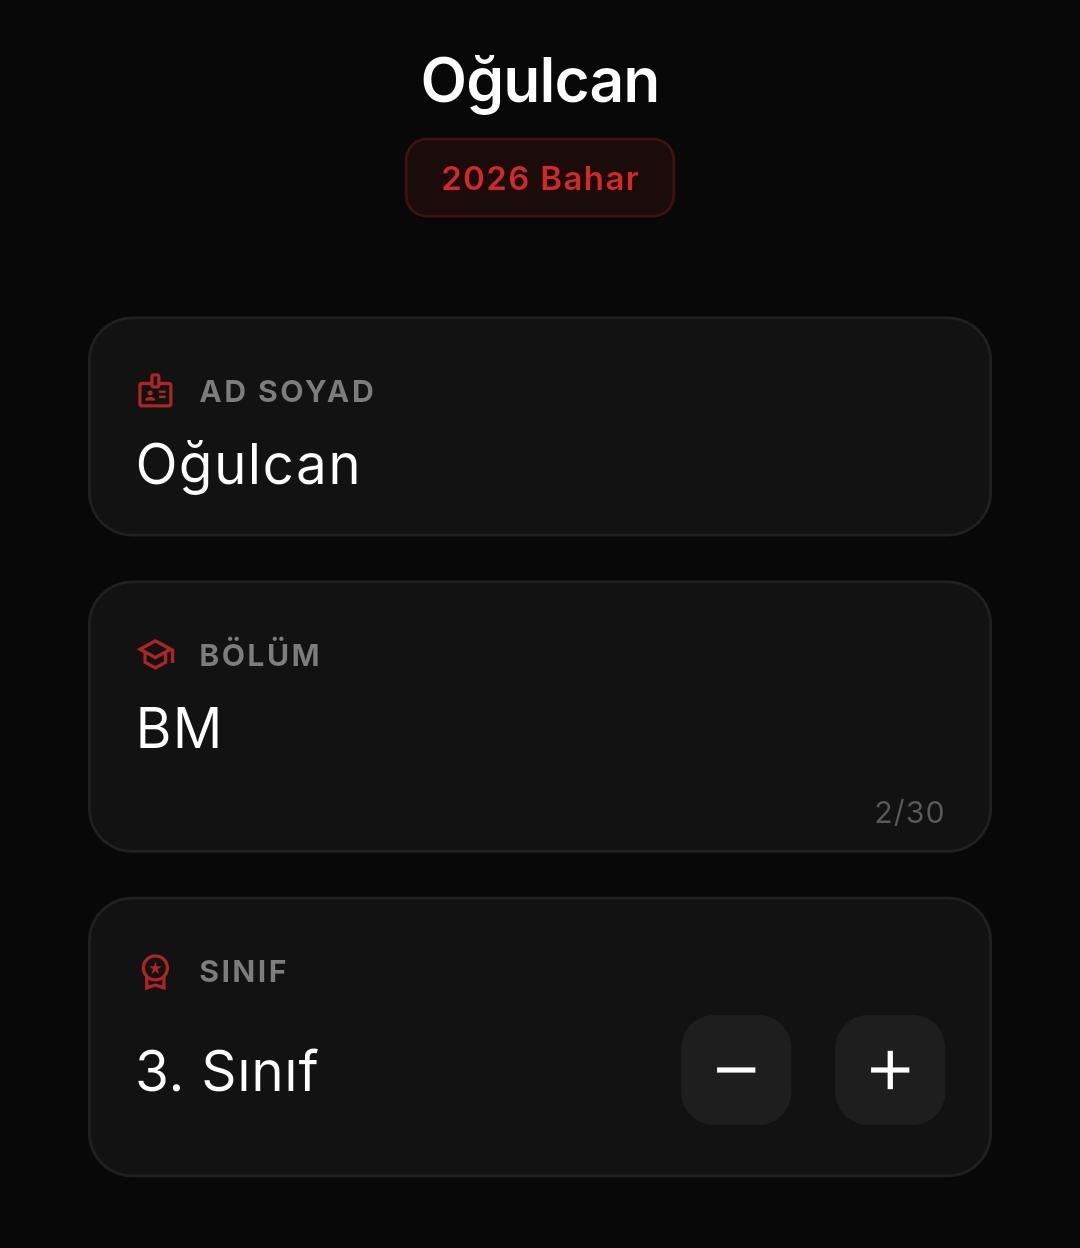
\includegraphics[height=9cm, keepaspectratio]{images/profile.jpeg}
    \caption{Profil Ekranı: Avatar, isim, bölüm ve sınıf bilgileri}
    \label{fig:profile}
\end{figure}

\begin{itemize}
    \item \textbf{Profil fotoğrafı:} Galeriden seçilir (maksimum 800px genişlik, \%85 kalite sıkıştırma). Fotoğraf eklenmemişse silüet simgesi görüntülenir.
    \item \textbf{Ad Soyad:} Maksimum 40 karakter.
    \item \textbf{Bölüm:} Maksimum 30 karakter; canlı karakter sayacı.
    \item \textbf{Sınıf:} 1--7 arası; +/- butonlarıyla ayarlanır.
    \item Girilen bilgiler kaydedilmeden \textbf{canlı önizleme} olarak gösterilir; aktif dönem rozeti avatar altında görünür.
\end{itemize}

\subsection{Ayarlar Ekranı}
\textbf{Dosya:} \texttt{features/settings/settings\_screen.dart}

\begin{figure}[H]
    \centering
    \begin{subfigure}[b]{0.42\textwidth}
        \centering
        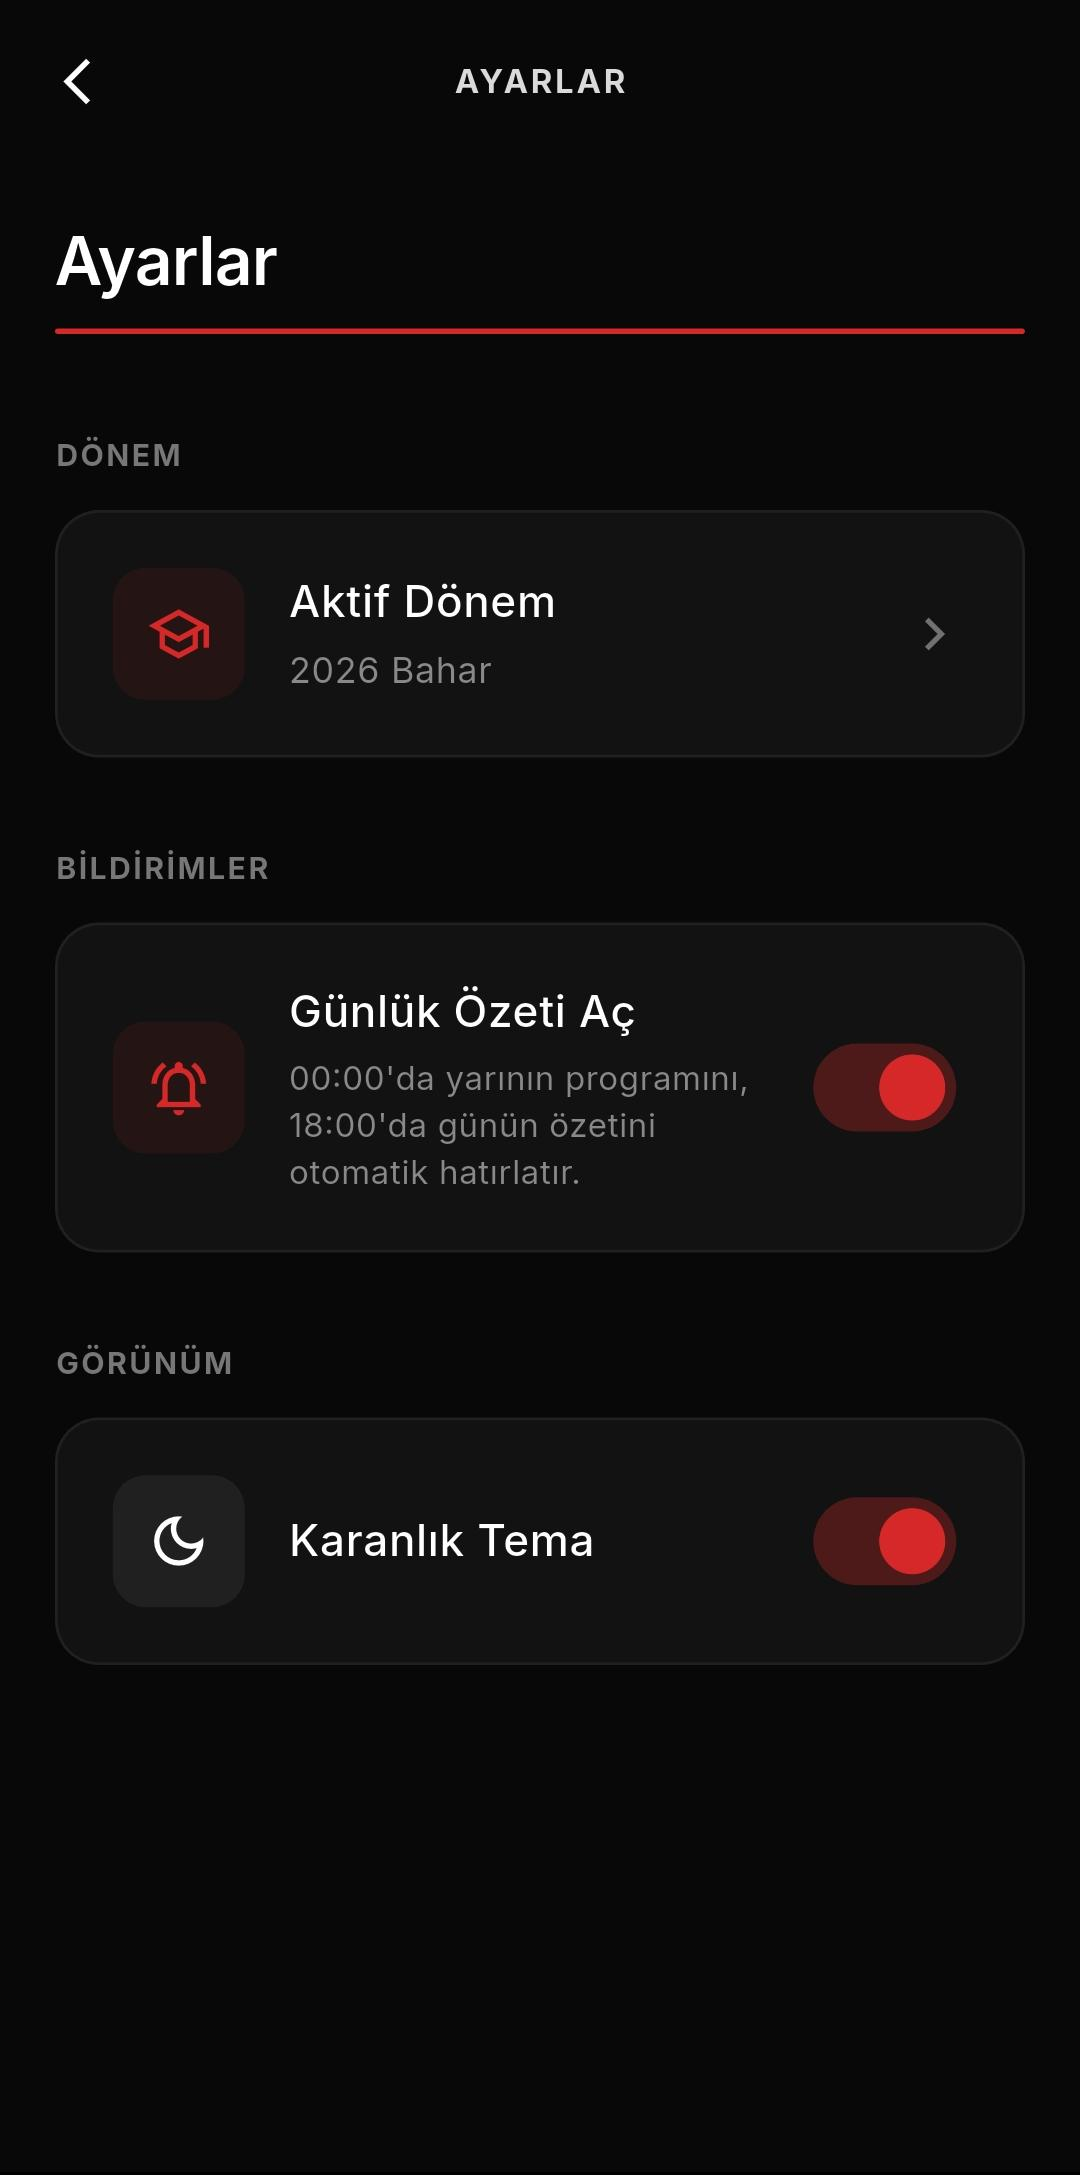
\includegraphics[height=8cm, keepaspectratio]{images/settings.jpeg}
        \caption{Ayarlar ana görünümü}
    \end{subfigure}
    \hfill
    \begin{subfigure}[b]{0.42\textwidth}
        \centering
        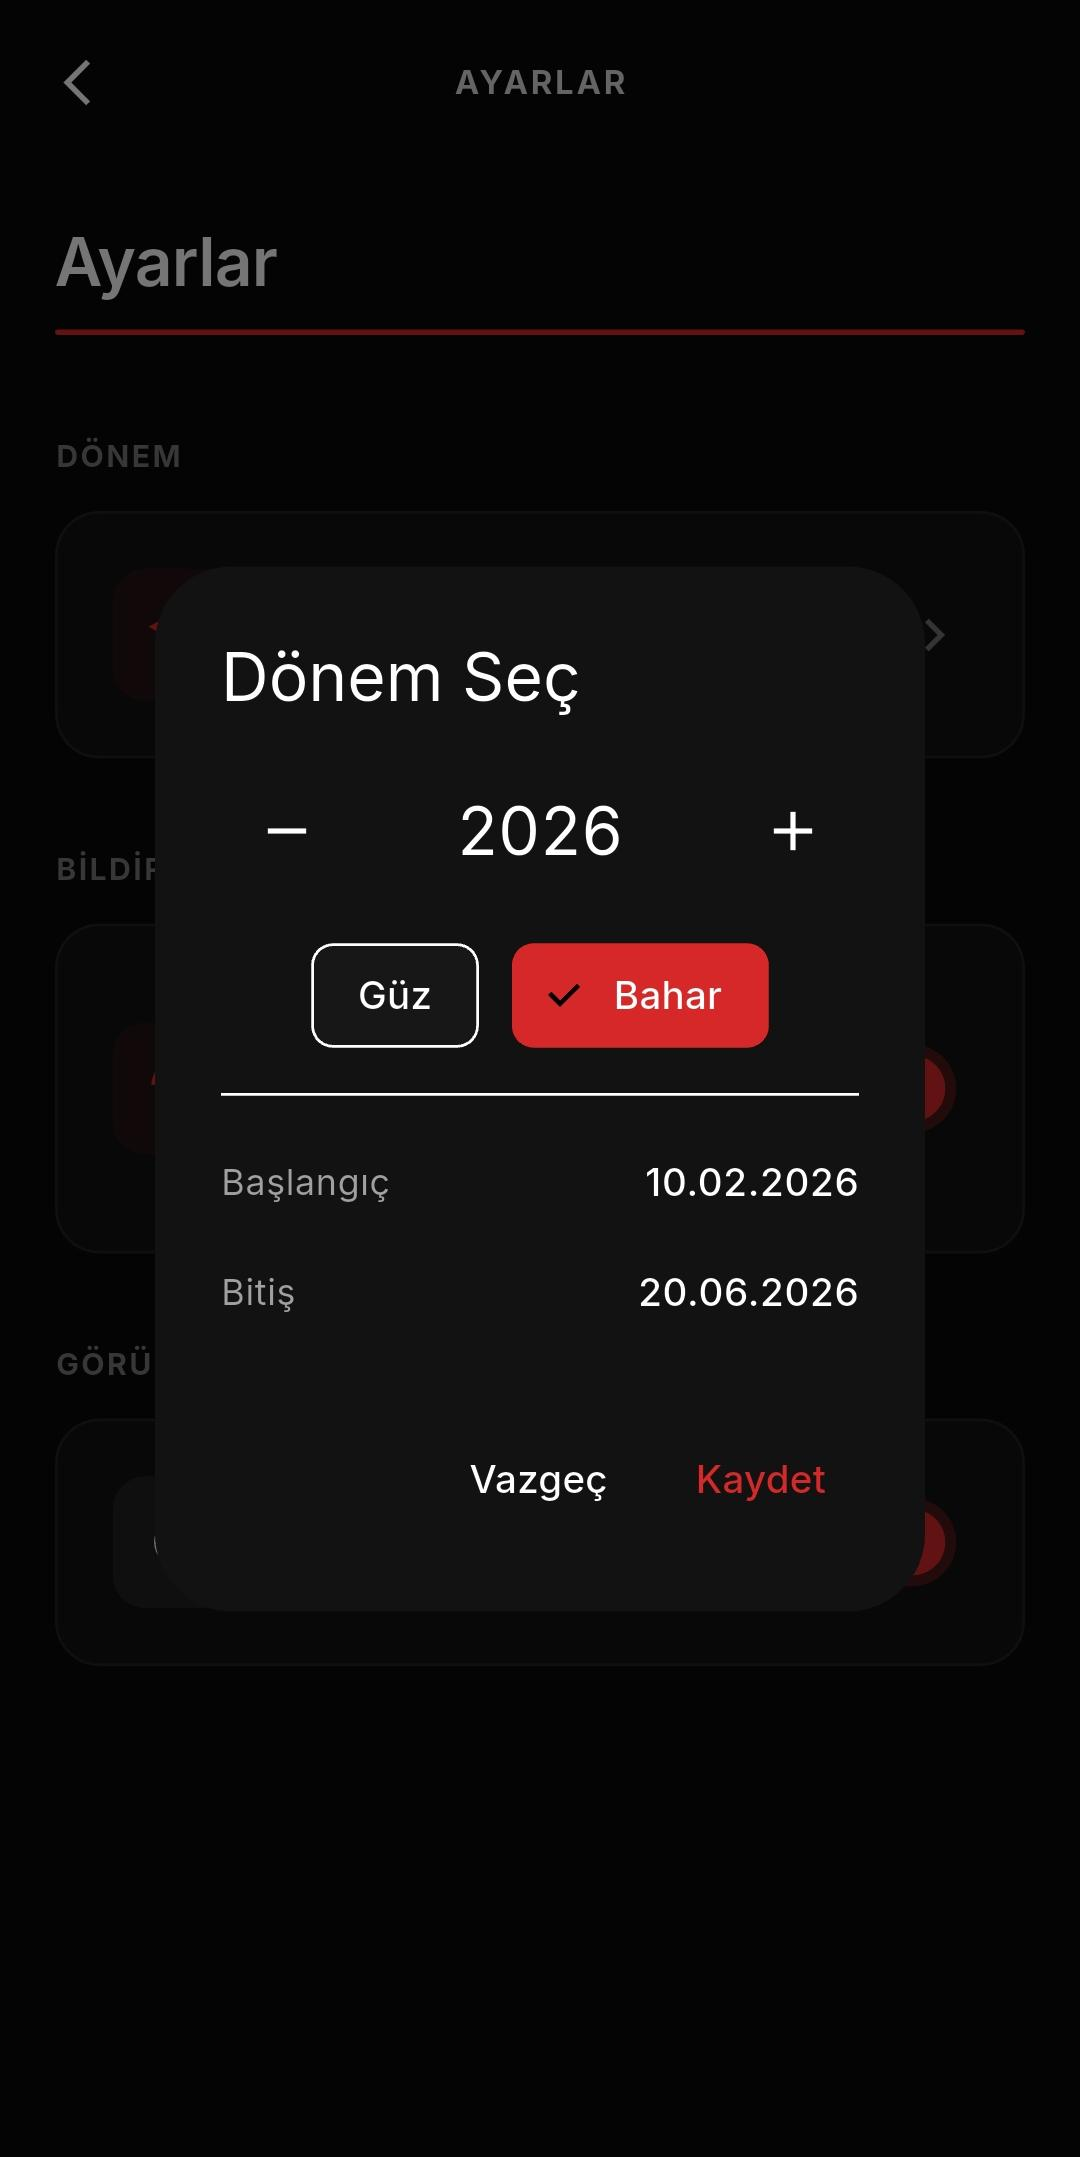
\includegraphics[height=8cm, keepaspectratio]{images/settings_term.jpeg}
        \caption{Dönem seçici dialog}
    \end{subfigure}
    \caption{Ayarlar Ekranı: Üç ayar kategorisi ve dönem seçici}
    \label{fig:settings}
\end{figure}

\begin{description}
    \item[DÖNEM] Aktif akademik dönem seçimi. Yıl, sezon (Güz/Bahar) ve isteğe bağlı başlangıç/bitiş tarihleri ayarlanır. Dönem değiştirildiğinde ana ekran yeni döneme ait verilerle yeniden yüklenir.
    \item[BİLDİRİMLER] ``Günlük Özeti Aç'' anahtarı ile 00:00 ve 18:00 hatırlatıcıları açılıp kapanır. İlk açılışta sistem bildirim izni talep edilir.
    \item[GÖRÜNÜM] Karanlık/Aydınlık tema geçişi. Tercih \texttt{SharedPreferences}'e kaydedilir; \texttt{ValueNotifier} aracılığıyla tüm uygulamaya anında yansır.
\end{description}

%% ============================================================
\section{Kullanıcı Akışları}
%% ============================================================

\subsection{İlk Kullanım Akışı}
\begin{enumerate}
    \item Uygulama açılır $\rightarrow$ Açılış ekranı (3,5 saniye animasyon)
    \item Ana ekran boş karşılama görünümü $\rightarrow$ \textbf{(+)} butonuna dokunulur
    \item Ders Ekleme ekranı: ders adı, saat, günler ve hak girilir $\rightarrow$ Kaydet
    \item Ana ekrana dönülür $\rightarrow$ Profil avatarına dokunulur
    \item Profil Ekranı: ad, bölüm, sınıf ve fotoğraf eklenir $\rightarrow$ Kaydet
\end{enumerate}

\subsection{Günlük Yoklama Akışı}
\begin{enumerate}
    \item Ana Ekran $\rightarrow$ ANA sekmesi $\rightarrow$ BUGÜN bölümü
    \item İlgili dersin kartındaki \textbf{GELDİM} veya \textbf{GELMEDİM} butonuna dokunulur
    \item ``Gelmedim'' seçilirse kalan hak otomatik olarak 1 azalır; 2 ve altına düşerse kırmızı uyarı rozeti gösterilir
    \item Yanlış işaret yapıldıysa \textbf{GERİ AL} butonuna dokunulur; hak iade edilir
\end{enumerate}

\subsection{Sınav Planlama Akışı}
\begin{enumerate}
    \item Ana Ekran $\rightarrow$ SINAVLAR sekmesi $\rightarrow$ \textbf{(+)} butonuna dokunulur
    \item Sınav Ekleme ekranı açılır; dersler üst şeritte etiket olarak listelenir
    \item Ders istenen takvim gününe sürükle-bırak yapılır
    \item Alt panel açılır: saat, yanına al ve not girilir $\rightarrow$ Kaydet
    \item SINAVLAR sekmesinden takvim veya ders notları görünümünde takip edilir
\end{enumerate}

\subsection{Dönem Değiştirme Akışı}
\begin{enumerate}
    \item Üst bardaki ayarlar (⚙) butonuna dokunulur
    \item \textbf{Dönem $\rightarrow$ Aktif Dönem}'e dokunulur $\rightarrow$ Dialog açılır
    \item Yıl, sezon seçilir; isteğe bağlı tarih aralığı belirlenir $\rightarrow$ Kaydet
    \item Ana ekran yeni döneme ait derslerle otomatik yeniden yüklenir
\end{enumerate}

\subsection{Bildirim Kurulum Akışı}
\begin{enumerate}
    \item Ayarlar $\rightarrow$ \textbf{Günlük Özeti Aç} anahtarına dokunulur
    \item Android/iOS bildirim izni istenir ve onaylanır
    \item Sonraki 7 gün için 00:00 ve 18:00 bildirimleri otomatik planlanır
    \item Belirli bir dersin bildirimini kapatmak için: ders kartı sola kaydırılır $\rightarrow$ \textbf{Sustur} seçilir
\end{enumerate}

%% ============================================================
\section{Arka Plan Servisleri}
%% ============================================================

\subsection{StorageService — Yerel Veri Saklama}
\textbf{Dosya:} \texttt{core/services/storage\_service.dart}

Tüm yerel veri erişimini tek noktada toplayan statik sınıftır. \texttt{SharedPreferences} üzerine JSON soyutlaması sağlar; UI katmanı doğrudan \texttt{SharedPreferences} ile iletişim kurmaz.

\begin{table}[H]
    \centering
    \caption{StorageService Depolama Anahtarları}
    \label{tab:storage}
    \renewcommand{\arraystretch}{1.3}
    \begin{tabularx}{\textwidth}{>{\ttfamily}l l X}
        \toprule
        \normalfont\textbf{Anahtar} & \textbf{Tip} & \textbf{İçerik} \\
        \midrule
        saved\_courses    & JSON List   & Tüm dönemlere ait dersler \\
        saved\_exams      & JSON List   & Tüm dönemlere ait sınavlar \\
        profile           & JSON Object & Öğrenci profil bilgileri \\
        active\_term      & JSON Object & Aktif dönem bilgisi \\
        morning\_reminder & Boolean     & Günlük bildirim açık/kapalı durumu \\
        \bottomrule
    \end{tabularx}
\end{table}

\textbf{Geriye dönük uyumluluk (migration):} Dönem alanı boş olan eski dersler otomatik olarak aktif döneme taşınır. Düz metin dönem kimlikleri (``2024-Güz'' string) yeni JSON formatına çözümlenir.

\subsection{NotificationService — Bildirim Servisi}
\textbf{Dosya:} \texttt{core/services/notification\_service.dart}

Tüm zamanlanmış bildirimleri yöneten statik sınıftır. \texttt{flutter\_local\_notifications} ve \texttt{timezone} paketleri kullanılır; saat dilimi \textbf{Europe/Istanbul}'a sabitlenmiştir.

\begin{table}[H]
    \centering
    \caption{Otomatik Bildirim Türleri}
    \label{tab:notif}
    \renewcommand{\arraystretch}{1.3}
    \begin{tabularx}{\textwidth}{l l X}
        \toprule
        \textbf{Saat} & \textbf{Başlık} & \textbf{İçerik} \\
        \midrule
        00:00 & Yarının Dersleri & Ertesi günün ders sayısı; ders yoksa ``Yarın Tatil'' mesajı; kritik hak uyarısı \\
        18:00 & Günü Tamamla & İşaretlenmemiş dersler hatırlatılır; tüm dersler işaretlendiyse teşvik mesajı \\
        \bottomrule
    \end{tabularx}
\end{table}

\textbf{Filtreleme kuralları:}
\begin{itemize}
    \item \texttt{notificationMuted: true} olan dersler dahil edilmez.
    \item Yalnızca aktif döneme ait dersler hesaba katılır.
    \item \texttt{HolidayService.isHoliday()} ile tatil günleri atlanır.
    \item Sonraki \textbf{7 gün} için bildirimler ileriye dönük planlanır.
\end{itemize}

\subsection{HolidayService — Tatil Servisi}
\textbf{Dosya:} \texttt{core/services/holiday\_service.dart}

Türkiye resmi tatil günlerini sağlayan statik sınıftır.

\begin{itemize}
    \item \textbf{Sabit milli bayramlar (7 adet):} Yılbaşı (1 Ocak), Ulusal Egemenlik ve Çocuk Bayramı (23 Nisan), Emek ve Dayanışma Günü (1 Mayıs), Atatürk'ü Anma ve Gençlik Bayramı (19 Mayıs), Demokrasi ve Milli Birlik Günü (15 Temmuz), Zafer Bayramı (30 Ağustos), Cumhuriyet Bayramı (29 Ekim).
    \item \textbf{Dini bayramlar:} Hicri takvime göre her yıl kaydığından Ramazan ve Kurban Bayramı için 2025--2027 yılları elle tanımlanmıştır.
    \item \texttt{isHoliday(date)} ve \texttt{nameFor(date)} metotlarıyla sorgulanır.
\end{itemize}

%% ============================================================
\section{Kod Mantığı ve Önemli Algoritmalar}
%% ============================================================

\subsection{Devamsızlık Hakkı Hesabı}

Yoklama işleminin çekirdeği \texttt{HomeScreen.\_markToday()} metodunda yer alır. Bir güne birden fazla işaret konulması önlenir; ``Gelmedim'' seçiminde hak sıfırda ise işlem reddedilir.

\begin{lstlisting}[caption={Yoklama işaretleme ve hak azaltma mantığı (home\_screen.dart)}, label={lst:mark}]
void _markToday(Course course, String status) {
  final today = DateTime.now();
  // Aynı gune birden fazla isaret engellenemez
  if (course.markFor(today) != null) return;

  setState(() {
    if (status == 'gelmedim') {
      if (course.rightsLeft <= 0) return; // Hak kalmadiysA islem yok
      course = course.copyWith(
        rightsLeft: course.rightsLeft - 1,
      );
    }
    course = course.copyWith(
      marks: {...course.marks, course.dayKey(today): status},
    );
    final idx = _allCourses.indexWhere((c) => c.id == course.id);
    _allCourses[idx] = course;
  });
  _persist(); // Kaydet + bildirimleri yeniden planla
}
\end{lstlisting}

\subsection{Türkçe Karakter Duyarlı Doğrulama}

Dart'ın yerleşik \texttt{toLowerCase()} metodu İngilizce kural uygular (İ $\rightarrow$ i değil; I $\rightarrow$ ı değil). Bu sorun özel yardımcı fonksiyon ile çözülmüştür:

\begin{lstlisting}[caption={Türkçe karakter duyarlı küçük harf dönüşümü (add\_course\_screen.dart)}, label={lst:trlower}]
String _trLower(String s) =>
    s.replaceAll('I', 'i')
     .replaceAll('İ', 'i') // buyuk I-noktalı → i
     .toLowerCase()
     .trim();

// Ayni donem icinde ayni isimli ders kontrolu
bool _isDuplicate(String name) {
  return _allCourses.any((c) =>
    c.id != widget.existing?.id &&
    _trLower(c.name) == _trLower(name) &&
    c.term == _activeTerm.id
  );
}
\end{lstlisting}

\subsection{Saat Tabanlı Sıralama}

Saati belirtilmemiş dersler her zaman listenin sonuna yerleştirilir:

\begin{lstlisting}[caption={Saate göre sıralama (course\_model.dart)}, label={lst:sort}]
int get sortMinutes {
  if (time.isEmpty) return 24 * 60 + 1; // Belirsiz saatler sona gider
  final parts = time.split(':');
  return int.parse(parts[0]) * 60 + int.parse(parts[1]);
}
\end{lstlisting}

\subsection{Veri Akışı Özeti}

\begin{enumerate}
    \item \texttt{HomeScreen.initState()} $\rightarrow$ \texttt{\_loadData()} $\rightarrow$ \texttt{StorageService}
    \item Herhangi bir kullanıcı eylemi $\rightarrow$ \texttt{setState()} ile yerel güncelleme
    \item \texttt{\_persist()} $\rightarrow$ \texttt{StorageService.saveCourses()} + bildirimleri yeniden planla
    \item Alt ekranlar (\texttt{CalendarScreen}, \texttt{ExamCalendarScreen}) veriyi \textit{parametre} olarak alır; depoyla doğrudan temas kurmaz
\end{enumerate}

%% ============================================================
\section{Tasarım ve Kullanıcı Deneyimi}
%% ============================================================

\subsection{Renk Paleti}

\begin{table}[H]
    \centering
    \caption{Uygulama Renk Paleti}
    \label{tab:renkler}
    \renewcommand{\arraystretch}{1.3}
    \begin{tabularx}{\textwidth}{l >{\ttfamily}l X}
        \toprule
        \textbf{Renk Adı} & \normalfont\textbf{Hex Kodu} & \textbf{Kullanım Amacı} \\
        \midrule
        Vurgu Kırmızısı & \#D62828 & CTA butonları, aktif sekmeler, kritik göstergeler \\
        Derin Kırmızı   & \#B81C1C & Kritik hak uyarıları (≤2 hak) \\
        Başarı Yeşili   & \#34C759 & ``Geldim'' durumu ve onay göstergeleri \\
        Sınav İndigo    & \#5B5BD6 & Sınav ekranı renk aksanı \\
        Arka Plan (Koyu) & \#080808 & Koyu tema arka planı \\
        Kart Yüzeyi (Koyu) & \#121212 & Koyu tema kart yüzeyi \\
        Arka Plan (Aydınlık) & \#F5F5F7 & Aydınlık tema arka planı \\
        \bottomrule
    \end{tabularx}
\end{table}

\subsection{Animasyonlar}

\begin{itemize}
    \item \textbf{Açılış:} Harf harf parlayan ışık efekti; \texttt{AnimationController} 2,5 saniyelik döngüde çalışır.
    \item \textbf{Aurora arka plan:} \texttt{CustomPainter} ile iki renk damlasının koordinatları sinüs dalgasıyla hareket ettirilir.
    \item \textbf{Nabız atan buton:} (+) ekleme butonunda sınır genişleme ve solma animasyonu.
    \item \textbf{Ders ekleme formu:} Her bölüm 80ms gecikmeli kademeli giriş animasyonu; toplam \textasciitilde{}600ms.
    \item \textbf{Sayfa geçişleri:} iOS tarzı kaydırma + solma; \texttt{CupertinoPageTransitionsBuilder} kullanılır.
    \item \textbf{Sekme geçişleri:} \texttt{AnimatedSwitcher} ile 280--850ms arası solma efekti.
\end{itemize}

\subsection{Performans Optimizasyonları}

\begin{itemize}
    \item \texttt{AutomaticKeepAliveClientMixin}: Sekme geçişlerinde takvim widget durumunu bellekte tutar; yeniden oluşturma yapılmaz.
    \item \texttt{RepaintBoundary}: Yoğun çizim gerektiren bileşenler izole edilerek gereksiz yeniden çizim engellenir.
    \item \textbf{Renk haritası önbelleği:} Takvim için renk haritası yalnızca ders listesi değiştiğinde yeniden hesaplanır.
\end{itemize}

%% ============================================================
\section{İşlev Özet Tablosu}
%% ============================================================

\begin{longtable}{>{\centering\bfseries}p{0.5cm} p{6.5cm} p{4cm} p{2.3cm}}
    \toprule
    \# & \textbf{İşlev} & \textbf{İlgili Ekran} & \textbf{Durum} \\
    \midrule
    \endfirsthead
    \toprule
    \# & \textbf{İşlev} & \textbf{İlgili Ekran} & \textbf{Durum} \\
    \midrule
    \endhead
    \bottomrule
    \endfoot
    1  & Ders ekleme                              & Ders Ekleme          & \textcolor{yesil}{\checkmark} Tamamlandı \\[2pt]
    2  & Ders düzenleme                           & Ders Ekleme          & \textcolor{yesil}{\checkmark} Tamamlandı \\[2pt]
    3  & Ders silme                               & Ana Ekran            & \textcolor{yesil}{\checkmark} Tamamlandı \\[2pt]
    4  & Günlük yoklama (Geldim / Gelmedim)       & Ana Ekran            & \textcolor{yesil}{\checkmark} Tamamlandı \\[2pt]
    5  & Devamsızlık hakkı otomatik hesabı        & Ana Ekran            & \textcolor{yesil}{\checkmark} Tamamlandı \\[2pt]
    6  & Yoklamayı geri alma                      & Ana Ekran            & \textcolor{yesil}{\checkmark} Tamamlandı \\[2pt]
    7  & Ders bildirimi susturma                  & Ana Ekran            & \textcolor{yesil}{\checkmark} Tamamlandı \\[2pt]
    8  & İsim ve günlük ders limiti doğrulama     & Ders Ekleme          & \textcolor{yesil}{\checkmark} Tamamlandı \\[2pt]
    9  & Ders takvimi (renkli nokta göstergeleri) & Ders Takvimi         & \textcolor{yesil}{\checkmark} Tamamlandı \\[2pt]
    10 & Resmi tatil gösterimi                    & Ders Takvimi         & \textcolor{yesil}{\checkmark} Tamamlandı \\[2pt]
    11 & Sınav ekleme (sürükle-bırak)             & Sınav Ekleme         & \textcolor{yesil}{\checkmark} Tamamlandı \\[2pt]
    12 & Sınav takvimi görünümü                   & Sınav Takvimi        & \textcolor{yesil}{\checkmark} Tamamlandı \\[2pt]
    13 & Ders bazlı sınav notları                 & Sınav Takvimi        & \textcolor{yesil}{\checkmark} Tamamlandı \\[2pt]
    14 & Sınav silme                              & Sınav Takvimi        & \textcolor{yesil}{\checkmark} Tamamlandı \\[2pt]
    15 & Profil ve fotoğraf yönetimi              & Profil               & \textcolor{yesil}{\checkmark} Tamamlandı \\[2pt]
    16 & Dönem (Güz/Bahar) yönetimi               & Ayarlar              & \textcolor{yesil}{\checkmark} Tamamlandı \\[2pt]
    17 & Otomatik bildirim (00:00 / 18:00)        & Ayarlar / Servis     & \textcolor{yesil}{\checkmark} Tamamlandı \\[2pt]
    18 & Karanlık / Aydınlık tema                 & Ayarlar              & \textcolor{yesil}{\checkmark} Tamamlandı \\[2pt]
    19 & Çevrimdışı veri saklama                  & Tüm Uygulama         & \textcolor{yesil}{\checkmark} Tamamlandı \\[2pt]
    \caption{Uygulama İşlev Özet Tablosu}
    \label{tab:ozetablo}
\end{longtable}

%% ============================================================
\section{Sonuç}
%% ============================================================

\textbf{Devamsızlık Takip} uygulaması, öğrencilerin akademik takiplerini kolaylaştırmak amacıyla geliştirilmiş, çevrimdışı çalışan ve tam işlevsel bir Flutter mobil uygulamasıdır.

Projenin öne çıkan katkıları şöyle özetlenebilir:

\begin{itemize}
    \item \textbf{Katmanlı mimari:} \texttt{core/} ve \texttt{features/} katmanlarının net ayrımı sayesinde kod bakımı ve genişletilmesi kolaylaşmaktadır.
    \item \textbf{Kullanıcı dostu arayüz:} Sürükle-bırak sınav ekleme, nabız atan butonlar, kademeli form animasyonları ve aurora arka plan gibi öğeler kullanıcı deneyimini ön plana çıkarmaktadır.
    \item \textbf{Akıllı bildirim sistemi:} Günlük 00:00 ve 18:00 hatırlatıcıları ile öğrenciler yoklamalarını unutmamaktadır.
    \item \textbf{Türkiye'ye özgü özellikler:} Istanbul saat dilimi, Türkçe karakter desteği ve resmi tatil entegrasyonu uygulamayı yerel kullanım için özelleştirmektedir.
    \item \textbf{Veri gizliliği:} Tüm veriler yalnızca kullanıcının cihazında saklandığından herhangi bir sunucu veya bulut riski bulunmamaktadır.
\end{itemize}

Uygulama, Flutter'ın sunduğu zengin widget ekosistemini, yerel veri saklama çözümlerini, bildirim sistemini ve özel animasyonları başarıyla bir araya getirerek kapsamlı bir öğrenci asistanı oluşturmuştur. Modüler yapısı sayesinde ileride not ortalaması hesaplama, ders programı PDF dışa aktarma veya bulut senkronizasyonu gibi yeni özellikler eklenmeye açıktır.

\vspace{1.5cm}
\begin{center}
    \color{gri}\rule{0.5\textwidth}{0.4pt}\\[0.5cm]
    \textit{Bu rapor, Artvin Çoruh Üniversitesi Mobil Programlama dersi kapsamında}\\[0.2cm]
    \textit{Doç.\@ Dr.\@ Hakan TEMİZ gözetiminde hazırlanmıştır.}\\[0.5cm]
    \textbf{Oğulcan Eyüp} \quad|\quad \textit{Haziran 2025}
\end{center}

\end{document}
